\chapter{Theoretische und technische Grundlagen}
\label{chap:theoretischeundtechnischegrundlagen}
Im Rahmen dieses Kapitels werden die maßgeblichen Technologien und Konzepte dargelegt, auf denen das entwickelte Modell basiert. Der Fokus liegt auf der automatisierten Objekterkennung, Textextraktion und strukturierten Informationsverarbeitung aus Gleisplänen.
\section{Grafische Gleispläne im Bahnkontext}
Die Modellierung einer Bahnanlage stellt eine komplexe Aufgabe dar, da diese typischerweise aus einer Vielzahl von Gleisabschnitten, Weichen und Signalen besteht. Die manuelle Erstellung eines Modells, das den physischen Details der Anlage entspricht, erfordert üblicherweise mehrere Wochen Arbeit. Dies hat signifikante Auswirkungen auf die Anwendbarkeit und den Umfang vieler Methoden.\cite{railroadstationdrawing}

Diese zeitintensive manuelle Arbeit motiviert den Einsatz automatisierter Verfahren zur Datenextraktion. Die folgenden Abschnitte legen die theoretischen Grundlagen dar, auf denen eine solche Automatisierung aufbauen kann.

\subsection{Grundlagen des Gleisplans}
Der Gleisplan bildet die fundamentale Datengrundlage für die Planung, den Bau und den operativen Betrieb von Bahnanlagen. Er repräsentiert die technische Infrastruktur und dient als visuelle Schnittstelle zwischen der physischen Außenanlage und der sicherungstechnischen Logik (Stellwerk).
\\
Gleispläne existieren in zwei Darstellungsformen \cite{Pachl}: maßstäbliche 
Lagepläne (topografisch, bautechnisch) und schematische Übersichtspläne 
(topologisch, sicherungstechnisch). Diese Arbeit fokussiert letztere, da sie 
die logischen Fahrwegbeziehungen priorisieren und die Grundlage für die Stellwerksplanung bilden.

Gleispläne enthalten drei Symbolkategorien: (1) Fahrwegelemente (Gleise, Weichen), 
(2) Sicherungstechnik (Signale, Achszähler), (3) Metadaten (Bezeichner, 
Kilometrierung). Jedes Element trägt eindeutige Labels zur Identifikation.

Obwohl diese Pläne in der heutigen Ingenieurspraxis mittels CAD-Systemen (Computer Aided Design) erstellt werden, liegt die primäre Herausforderung für eine automatisierte Auswertung nicht im Dateiformat, sondern in der korrekten semantischen Interpretation dieser abstrahierten Symbolik und ihrer logischen Verknüpfung \cite{Pachl}.

\begin{figure}[H]
    \centering
    \includegraphics[width=1\textwidth]{images/tracklayout2.png} 
    \caption{Ausschnitt eines schematischen Gleisplans mit Darstellung von Signalen, Weichen und Gleisbezeichnungen (Beispielhafte Darstellung) aus Quelle \cite{railroadstationdrawing}}
    \label{fig:gleisplan_schema}
\end{figure}

\subsection{Bahntechnische Symbole und ihre Klassifikation}
\label{sec:Bahntechnischesymbole}
In den Gleisplänen kommen zahlreiche Symbole zum Einsatz, um die verschiedenen technischen Objekte, Anlagenkomponenten und zusätzlichen Informationen übersichtlich darzustellen. Diese Symboldarstellung dient nicht nur der Visualisierung der Gleiskomponenten, sondern bildet auch die Grundlage für Planung, Projektierung, Dokumentation und spätere Anwendung. \cite{signallayout} Da der Gleisplan eine zentrale Schnittstelle zwischen technischer Planung, 
betrieblicher Umsetzung und sicherheitstechnischen Systemen darstellt, ist eine präzise, klare und einheitliche Symbolklassifizierung notwendig. Die für diese Arbeit relevanten Symbolklassen gliedern sich in drei funktionale 
Kategorien (siehe Tabelle \ref{tab:symbol_categories}):

\begin{table}[h]
\centering
\begin{tabular}{|p{3.5cm}|p{11.5cm}|}
\hline
\textbf{Kategorie} & \textbf{Elemente und Funktion} \\
\hline
Infrastruktur & \textbf{Signale}: Fahrterlaubnis und Geschwindigkeitsvorgabe\cite{Pachl}. 
\textbf{Weichen}: Fahrwegverzweigungen\cite{Pachl}. \\
\hline
Zugbeeinflussung & \textbf{Balisen}: Übertragung von Fahrt-/Haltinformationen, 
Geschwindigkeitsinformationen und weiteren Daten des Stellwerkes an den Zug\cite{Pachl}. 
\textbf{Gleismagnete}: Übertragung von Fahrt-/Haltinformationen, 
Geschwindigkeitsinformationen und weiteren Daten des Stellwerkes an den Zug\cite{Pachl}. 
\textbf{Gleiskoppelspulen}: Übertragung von Fahrt-/Haltinformationen, 
Geschwindigkeitsinformationen und weiteren Daten des Stellwerkes an den Zug\cite{Pachl}. \\
\hline
Belegungserkennung & \textbf{Isolierstöße}: Elektrische Gleistrennung zur 
Definition von Gleisstromkreisen für die Belegungserkennung\cite{Pachl}. 
\textbf{Achszähler}: Zählpunktbasierte Belegungserkennung durch Erfassung 
ein- und ausfahrender Achsen\cite{Pachl}. \\
\hline
Metadaten & \textbf{Positionsangaben}: Kilometrierung, Lagepunkte\cite{DB2008Regelwerk}. 
\textbf{Gleisabschnittsnamen}: Eindeutige Gleisidentifikation\cite{DB2008Regelwerk}. \\
\hline
\end{tabular}
\caption{Klassifikation bahntechnischer Symbole}
\label{tab:symbol_categories}
\end{table}

Die automatisierte Analyse visueller Informationen bildet das Fundament zahlreicher technischer Anwendungen von der Qualitätskontrolle in der industriellen Fertigung über die medizinische Bildanalyse bis hin zur autonomen Navigation. Während Menschen mühelos in der Lage sind, Objekte in Bildern zu identifizieren und zu lokalisieren, erfordert die Replikation dieser Fähigkeit in Maschinen die Lösung komplexer Teilprobleme. Historisch wurde diese Aufgabe durch explizite Programmierung von Erkennungsregeln adressiert. Der konzeptionelle Durchbruch gelang durch maschinelles Lernen, insbesondere durch tiefe neuronale Netze, die relevante Merkmale selbstständig aus Trainingsdaten extrahieren können \cite{LeCun1998_GradientBasedLearning,Krizhevsky2012_AlexNet}.

Für technische Anwendungen wie die Analyse von Konstruktionszeichnungen oder Gleisplänen manifestieren sich spezifische Herausforderungen, die über die Verarbeitung natürlicher Fotografien hinausgehen. Im Folgenden werden zunächst die domänenspezifischen Anforderungen technischer Zeichnungen erläutert, bevor die grundlegenden methodischen Ansätze der Objekterkennung systematisch hergeleitet werden. Das Kapitel folgt dabei einer Progression vom Allgemeinen zum Spezifischen: Ausgehend von universellen Erkennungsprinzipien wird schrittweise die Anwendung auf bahntechnische Gleispläne konkretisiert.

\subsection{Objekterkennung in technischen CAD-Zeichnungen}
\label{subsec:cad_spezifisch}

Im Gegensatz zu natürlichen Szenen weisen technische Konstruktionszeichnungen spezifische Charakteristika auf, die dedizierte Lösungsansätze erfordern. Diese domänenspezifischen Besonderheiten haben direkten Einfluss auf die Wahl geeigneter Erkennungsverfahren und definieren die in Kapitel \ref{chap:anforderungen} formulierten funktionalen Anforderungen an das System.

\subsubsection{Domänenspezifische Eigenschaften}

Technische Zeichnungen unterscheiden sich fundamental von natürlichen Bildern in ihrer Entstehung und Struktur. CAD-Systeme (Computer-Aided Design) erzeugen vektorbasierte Repräsentationen, die geometrische Primitive wie Linien, Kreise und Polylinien sowie zugeordnete Metadaten enthalten. Die Konvertierung in Rasterformate (PDF, PNG) für ML-basierte Analyse führt jedoch zu einem Informationsverlust hinsichtlich topologischer Beziehungen und semantischer Layer-Informationen. Topologische Beziehungen beschreiben die Verbindungsstruktur zwischen Elementen -- etwa welche Gleisabschnitte durch eine Weiche verbunden sind oder welches Signal zu welchem Gleis gehört. Semantische Layer-Informationen kodieren die funktionale Zuordnung von Objekten zu Kategorien wie Gleisführung, Signaltechnik oder Oberleitung. Bei der Rasterisierung werden diese Strukturinformationen eliminiert; das Bild wird zu einer Ansammlung von Pixeln ohne inhärente Bedeutung. Diese Transformation von strukturierten zu unstrukturierten Daten motiviert den Einsatz von Deep-Learning-Verfahren, die robuste Mustererkennung auch ohne explizite topologische Information ermöglichen.

Bahntechnische Symbole folgen standardisierten Bibliotheken gemäß EN-Normen oder kundenspezifischen Richtlinien. Die Variabilität innerhalb einer Symbolklasse ist somit deutlich geringer als bei natürlichen Objekten wie Fahrzeugen oder Personen, jedoch erschweren kundenspezifische Anpassungen die Generalisierung über verschiedene Planungsunternehmen hinweg. Ein durchschnittlicher Bahnhofsgleisplan enthält zwischen 500 und 2000 individuelle Symbole auf einer Fläche von wenigen Quadratmetern, was eine deutlich höhere Objektdichte als in typischen Computer-Vision-Benchmark-Datensätzen wie COCO \cite{Lin2014_COCO} oder Pascal VOC \cite{Everingham2010_PascalVOC} darstellt. Zum Vergleich: COCO-Bilder enthalten im Durchschnitt 7 bis 10 Objekte, während ein Gleisplanausschnitt von vergleichbarer Pixelgröße 50 bis 100 Symbole aufweisen kann.

Anders als bei Objekten mit kanonischer Orientierung -- etwa Straßenverkehrsschilder (typischerweise frontal) oder Fußgänger (vertikal stehend) -- können bahntechnische Symbole und Textannotationen entlang der Gleisachsen in beliebigen Winkeln orientiert sein. Ein Weichensymbol kann beispielsweise in 16 verschiedenen Rotationen auftreten, die jeweils 22,5° Schritte zwischen 0° und 360° abdecken. Signale werden parallel zur Gleisachse positioniert, Gleisnummern folgen der Krümmung des Gleises. Diese Rotationsvariabilität ohne bevorzugte Ausrichtung erfordert rotationsinvariante Detektionsarchitekturen, deren Notwendigkeit in Abschnitt \ref{sec:obb} detailliert erläutert wird.

\subsubsection{Stand der Forschung}

Die Anwendung von Machine Learning auf technische Zeichnungen ist ein aktives Forschungsfeld mit Anwendungen in verschiedenen Ingenieurdisziplinen. Ahmed et al. \cite{Ahmed2011} entwickelten frühe Ansätze zur automatischen Segmentierung von architektonischen Grundrissen unter Verwendung morphologischer Operationen und Hough-Transformation. Moreno-García et al. \cite{Moreno2019} entwickelten ein umfassendes Framework zur Digitalisierung komplexer technischer Zeichnungen und demonstrierten die Überlegenheit von Deep-Learning-Ansätzen gegenüber klassischen Feature-Engineering-Methoden. Rahul et al. \cite{Rahul2019} extrahierten Informationen aus P\&ID-Diagrammen der Prozessindustrie mittels Faster R-CNN und erreichten dabei mean Average Precision-Werte von über 85\%.

Jamieson et al. \cite{Jamieson2024} liefern eine umfassende Übersicht über Deep-Learning-Methoden für Engineering-Diagramme und identifizieren als zentrale Herausforderungen die hohe Variabilität kundenspezifischer Symbolbibliotheken, den Mangel an annotierten Trainingsdaten sowie die Notwendigkeit rotationsinvarianter Detektionsverfahren. Für den bahntechnischen Bereich existieren bisher hauptsächlich proprietäre Lösungen einzelner Eisenbahnunternehmen ohne publizierte wissenschaftliche Evaluierung. Die vorliegende Arbeit adressiert diese Forschungslücke durch Entwicklung und Evaluation eines prototypischen Systems auf Basis moderner One-Stage-Detektoren.



\subsection{Entwicklung der Objekterkennung}
Die erwähnten Detektionsverfahren basieren auf \textit{Deep Learning}, einer Form des maschinellen Lernens, bei der künstliche neuronale Netze -- insbesondere \textit{Convolutional Neural Networks} (CNNs) -- 
relevante Merkmale automatisch aus Trainingsbildern lernen \cite{neuralnetwork}. Im Gegensatz zu klassischen Verfahren, bei denen Erkennungsmerkmale manuell definiert werden müssen, ermöglichen 
CNNs die End-to-End-Optimierung des gesamten Erkennungssystems. Die folgenden Abschnitte beschreiben zunächst die historische Entwicklung 
dieser Technologie, bevor spezialisierte Architekturen für die Objekterkennung detailliert werden.
Die Objekterkennung hat sich von regelbasierten Verfahren über klassisches 
maschinelles Lernen zu Deep-Learning-Ansätzen entwickelt 
\cite{Zou2019_ObjectDetectionSurvey}. Für die vorliegende Arbeit werden 
ausschließlich CNN-basierte Detektoren eingesetzt, da diese bei technischen 
Zeichnungen signifikant höhere Erkennungsraten erreichen als klassische 
Verfahren (vgl. Kapitel~\ref{chap:konzeption}, Tabelle~\ref{tab:Alternative_Detection}).

\subsection{Architekturen für Deep-Learning-basierte Objekterkennung}
\label{subsec:dl_architekturen}

Die Implementierung von CNN-basierten Objektdetektoren lässt sich in zwei Architekturparadigmen unterteilen, die sich in ihrer Balance zwischen Detektionsgenauigkeit und Recheneffizienz unterscheiden. Die Wahl der Architektur hat direkte Auswirkungen auf die Praxistauglichkeit des Systems.

\subsubsection{Zweistufige vs. einstufige Detektoren}

Zweistufige Detektoren wie Faster R-CNN \cite{Ren2015_FasterRCNN} separieren den Erkennungsprozess konzeptionell in zwei aufeinanderfolgende Phasen. Zunächst generiert ein Region Proposal Network (RPN) zwischen 100 und 300 Kandidatenregionen, die potenziell Objekte enthalten könnten. Diese Regionen werden anschließend durch ein separates Klassifikationsnetzwerk evaluiert, das sowohl die Objektklasse bestimmt als auch die Bounding-Box-Koordinaten verfeinert. Der Vorteil liegt in hoher Detektionspräzision, insbesondere bei kleinen oder teilweise verdeckten Objekten. Die sequenzielle Verarbeitung hunderter Kandidatenregionen führt jedoch zu Bildraten von lediglich 5 bis 10 Bildern pro Sekunde (Frames Per Second, FPS) auf moderner GPU-Hardware (Graphics Processing Unit).

Für die Gleisplananalyse erweist sich diese Geschwindigkeit als kritisch. Ein durchschnittlicher Plan umfasst nach der Kachelungsstrategie (siehe Abschnitt \ref{subsubsec:tiling_strategie}) zwischen 150 und 300 Bildausschnitte. Während YOLO-Modelle typischerweise mit Eingangsgrößen von 640×640 oder 1024×1024 Pixeln arbeiten, werden für die Gleisplananalyse aufgrund der sehr kleinen Symbolgrößen Kacheln von 2048×2048 Pixeln verwendet (Details zur Kachelungsstrategie in Abschnitt \ref{subsubsec:tiling_strategie}). Bei einer Verarbeitungszeit von 100 bis 200 Millisekunden pro Kachel würde die Gesamtanalyse zwischen 15 Sekunden und 4 Minuten dauern. 

Einstufige Detektoren wie YOLO (You Only Look Once) \cite{redmon2016lookonceunifiedrealtime} adressieren diese Geschwindigkeitsproblematik durch eine fundamental andere Strategie. YOLO unterteilt das Eingabebild in ein regelmäßiges Raster von Zellen (beispielsweise 13×13 oder 26×26 Zellen bei kleineren Eingabegrößen, bzw. entsprechend größere Raster bei höheren Auflösungen). Für jede Zelle sagt das Netz in einem einzigen Vorwärtsdurchlauf direkt mehrere Aspekte voraus: Liegt in dieser Zelle ein Objekt? Wenn ja, welcher Objektklasse gehört es an? Wie hoch ist die Konfidenz dieser Vorhersage? Und wo genau innerhalb der Zelle befindet sich das Objekt? Diese parallele Verarbeitung aller Bildbereiche ermöglicht Inferenzgeschwindigkeiten von 40 bis über 100 Bildern pro Sekunde \cite{yolov8_ultralytics}. Moderne Varianten wie YOLOv8 erreichen durch architektonische Verbesserungen -- insbesondere Feature Pyramid Networks (FPN) \cite{Lin2017_FPN} für Multi-Scale-Detektion und verbesserte Loss-Funktionen -- vergleichbare oder sogar überlegene Präzision gegenüber zweistufigen Detektoren bei Beibehaltung der Echtzeitfähigkeit.

Die Abwägung zwischen beiden Paradigmen muss im Kontext der Anwendungsanforderungen erfolgen. Für technische Gleispläne mit gut sichtbaren, scharf gerenderten Symbolen rechtfertigt die hohe Verarbeitungsgeschwindigkeit marginale Genauigkeitseinbußen. Einstufige Architekturen können bei technischen Zeichnungen vergleichbare Präzision erreichen (die konkrete Evaluation erfolgt in Kapitel~\ref{chap:evaluation}).

Abbildung \ref{fig:two_stage_vs_one_stage} illustriert den fundamentalen Unterschied zwischen beiden Architekturparadigmen. Faster R-CNN generiert zunächst mehrere hundert Kandidatenregionen mittels RPN, die anschließend sequenziell klassifiziert werden müssen. YOLO hingegen sagt in einem einzigen Vorwärtsdurchlauf direkt die Bounding Boxes und Klassen voraus, was zu einer Beschleunigung um den Faktor 5 führt. Für die Analyse eines typischen Gleisplans mit 200 gekachelten Bildausschnitten (je 2048×2048 Pixel) reduziert sich die Gesamtverarbeitungszeit von etwa 4 Minuten (Faster R-CNN) auf unter 5 Sekunden (YOLO).

% ABBILDUNG 3.2: Two-Stage vs One-Stage
\begin{figure}[H]
\centering
\begin{tikzpicture}[
    node distance=1.5cm,
    box/.style={rectangle, draw, thick, minimum width=2.8cm, minimum height=1cm, align=center, font=\footnotesize},
    arrow/.style={->, >=stealth, thick}
]
    % LEFT: Two-Stage
    \node[box, fill=blue!15] (img1) {Eingabebild\\$1024 \times 1024$ px};
    \node[box, fill=yellow!25, below=of img1] (rpn) {Region Proposal\\Network\\$\sim$300 Kandidaten};
    \node[box, fill=orange!20, below=of rpn] (class1) {Klassifikation\\pro Region};
    \node[box, fill=green!20, below=of class1] (out1) {Detektionen};
    
    \draw[arrow] (img1) -- (rpn);
    \draw[arrow] (rpn) -- (class1);
    \draw[arrow] (class1) -- (out1);
    
    \node[left=0.6cm of rpn, align=right, font=\scriptsize\bfseries] (label1) {Two-Stage\\(Faster R-CNN)};
    \node[below=0.15cm of label1, align=right, font=\tiny, text width=2.2cm] {$\sim$8 FPS\\Hohe Präzision\\4 Min/Gleisplan};
    
    % RIGHT: One-Stage
    \begin{scope}[xshift=6.5cm]
        \node[box, fill=blue!15] (img2) {Eingabebild\\$1024 \times 1024$ px};
        \node[box, fill=green!20, below=3.2cm of img2] (direct) {Direkte Vorhersage\\(Grid-basiert)};
        \node[box, fill=green!20, below=of direct] (out2) {Detektionen};
        
        \draw[arrow] (img2) -- (direct);
        \draw[arrow] (direct) -- (out2);
        
        \node[right=0.6cm of direct, align=left, font=\scriptsize\bfseries] (label2) {One-Stage\\(YOLO)};
        \node[below=0.15cm of label2, align=left, font=\tiny, text width=2.2cm] {$\sim$40 FPS\\Echtzeitfähig\\5 Sek/Gleisplan};
    \end{scope}
    
    % Comparison arrow
    \draw[<->, >=stealth, thick, red!70!black] (out1.south) ++ (0,-0.4) -- ++ (6.5,0) 
        node[midway, below, font=\scriptsize, align=center] {Faktor 5 schneller};
\end{tikzpicture}
\caption{Architekturvergleich zwischen zweistufigen und einstufigen Objektdetektoren.}
\label{fig:two_stage_vs_one_stage}
\end{figure}

\subsection{Modelltraining}

Das Training erfolgt supervised mit annotierten Bounding Boxes. Die konkreten 
Trainingsparameter und Augmentationsstrategien werden in 
Kapitel~\ref{chap:implementierung}, Abschnitt \ref{subsec:Modelltraining} dokumentiert.

\subsection{Evaluationsmetriken}
\label{subsec:evaluationsmetriken}

Die Bewertung von Objektdetektoren erfordert standardisierte Metriken, die sowohl Lokalisierungsgenauigkeit als auch Klassifikationsgüte quantifizieren. Im Gegensatz zu einfachen Klassifikationsproblemen müssen Detektoren beide Aspekte simultan korrekt vorhersagen. Die nachfolgenden Metriken bilden die Grundlage für die in Kapitel \ref{chap:evaluation} präsentierte Systemevaluation.

\subsubsection{Intersection over Union}

Die Intersection over Union (IoU) \cite{Everingham2010_PascalVOC} quantifiziert den Überlappungsgrad zwischen vorhergesagter Box $B_{\text{pred}}$ und Ground-Truth-Box $B_{\text{gt}}$:

\begin{equation}
\text{IoU}(B_{\text{pred}}, B_{\text{gt}}) = 
\frac{\text{Area}(B_{\text{pred}} \cap B_{\text{gt}})}
{\text{Area}(B_{\text{pred}} \cup B_{\text{gt}})}
\end{equation}

Der IoU-Wert liegt im Intervall $[0, 1]$, wobei 0 keine Überlappung und 1 perfekte Übereinstimmung signalisiert. In der Praxis gilt eine Detektion als korrekt, wenn $\text{IoU} \geq 0.5$ -- das heißt, die Überlappung muss mindestens die Hälfte der Gesamtfläche betragen. Dieser Schwellenwert reflektiert einen Kompromiss zwischen Forderung nach Präzision und Toleranz gegenüber geringfügigen Positionsabweichungen. Für präzisionskritische Anwendungen werden teilweise höhere Schwellen (0.75 oder 0.9) verwendet \cite{Lin2014_COCO}.

Abbildung \ref{fig:iou_visualization} veranschaulicht diese Berechnung anhand eines konkreten Beispiels. Die grüne Box repräsentiert die Ground-Truth-Position eines Symbols, wie sie von einem menschlichen Annotator markiert wurde. Die blaue Box stellt die Vorhersage des Detektors dar. Die Schnittfläche (rot schraffiert) entspricht der Fläche, in der beide Boxen überlappen. Die Vereinigungsfläche (durch die gestrichelte schwarze Linie umrandet) umfasst alle Bereiche, die von mindestens einer der beiden Boxen abgedeckt werden. Im dargestellten Fall beträgt die IoU etwa 0.28, was unterhalb der üblichen Schwelle von 0.5 liegt. Obwohl visuell erkennbar ist, dass der Detektor das richtige Objekt identifiziert hat, wird die Detektion aufgrund der ungenügenden Lokalisierung als Fehldetektion gewertet. Dies verdeutlicht die Strenge der IoU-Metrik: Nicht nur die korrekte Objektklasse, sondern auch eine präzise Lokalisierung ist erforderlich.

\begin{figure}[H]
\centering
\begin{tikzpicture}[scale=1.1]
    % Ground Truth (grün)
    \draw[thick, green!70!black, fill=green!20, opacity=0.7] (1,1) rectangle (5,3.5);
    \node[green!70!black, font=\small\bfseries] at (0.5, 3.8) {Ground Truth};
    
    % Prediction (blau)
    \draw[thick, blue!70!black, fill=blue!20, opacity=0.7] (2.5,1.8) rectangle (6.5,4.3);
    \node[blue!70!black, font=\small\bfseries] at (4.5, 4.6) {Vorhersage};
    
    % Intersection (rot)
    \begin{scope}
        \clip (1,1) rectangle (5,3.5);
        \fill[pattern=north east lines, pattern color=red!80!black, opacity=0.8] 
            (2.5,1.8) rectangle (6.5,4.3);
    \end{scope}
    \draw[thick, red!80!black] (2.5,1.8) rectangle (5,3.5);
    \node[red!80!black, font=\small\bfseries] at (3.75, 2.65) {Schnitt};
    
    % Union (gestrichelt)
    \draw[thick, dashed, black] (1,1) -- (1,3.5) -- (2.5,3.5) -- (2.5,4.3) -- 
        (6.5,4.3) -- (6.5,1.8) -- (5,1.8) -- (5,1) -- cycle;
    
    \node[below, font=\small] at (3.75, 0.3) {$\text{IoU} \approx 0.28$ (zu niedrig, gilt als Fehldetektion)};
\end{tikzpicture}
\caption{Visualisierung der Intersection over Union (IoU)-Metrik.}
\label{fig:iou_visualization}
\end{figure}

\subsubsection{Precision, Recall und Mean Average Precision}

Basierend auf der IoU-Schwelle werden Detektionen klassifiziert: True Positives (TP, korrekte Detektionen mit IoU $\geq$ 0.5), False Positives (FP, Falschdetektionen oder korrekte Klasse aber IoU $<$ 0.5) und False Negatives (FN, übersehene Objekte). Daraus ergeben sich Precision und Recall \cite{Everingham2010_PascalVOC}:

\begin{equation}
\text{Precision} = \frac{TP}{TP + FP}, \quad 
\text{Recall} = \frac{TP}{TP + FN}
\end{equation}

Die Precision gibt an, welcher Anteil der vom Detektor gemeldeten Objekte tatsächlich korrekt ist. Ein hoher Precision-Wert bedeutet wenige Fehlalarme. Der Recall misst, welcher Anteil der im Bild tatsächlich vorhandenen Objekte vom Detektor gefunden wurde. Ein hoher Recall-Wert bedeutet, dass wenige Objekte übersehen werden. Beide Metriken stehen typischerweise in einem Trade-off: Durch Erhöhung der Konfidenzschwelle kann Precision verbessert werden, jedoch auf Kosten des Recalls.

Für Gleisplanerkennung ist insbesondere der Recall kritisch. Ein übersehenes Signal oder eine fehlende Weichenkennzeichnung kann zu gravierenden Fehlern in der nachfolgenden Planung führen -- etwa falsche Berechnung von Gleiskapazitäten oder Sicherheitsrisiken. Falschdetektionen (niedrige Precision) sind weniger kritisch, da sie in der Validierungsphase (siehe Abschnitt \ref{sec:datenvalidierung}) durch regelbasierte Filter und Plausibilitätsprüfungen eliminiert werden können. Ein falsch detektiertes Signal an einer unmöglichen Position (etwa mitten auf einem Gleis ohne Haltemöglichkeit) wird durch die semantische Validierung verworfen.

Die Mean Average Precision (mAP) \cite{Everingham2010_PascalVOC,Lin2014_COCO} aggregiert die Erkennungsgüte über alle Objektklassen und verschiedene Konfidenzschwellen. Für jede Klasse wird zunächst die Average Precision (AP) als Fläche unter der Precision-Recall-Kurve berechnet. Diese Kurve entsteht, indem die Konfidenzschwelle variiert wird: Bei niedriger Schwelle werden viele Objekte detektiert (hoher Recall, niedrige Precision), bei hoher Schwelle nur sehr sichere Detektionen (niedriger Recall, hohe Precision). Die mAP ist der Mittelwert über alle Klassen:

\begin{equation}
\text{mAP} = \frac{1}{N} \sum_{i=1}^{N} \text{AP}_i
\end{equation}

wobei $N$ die Anzahl der Objektklassen bezeichnet. Üblich ist die Angabe von mAP@0.5 (IoU-Schwelle 50\%) sowie mAP@[0.5:0.95] (Mittelwert über IoU-Schwellen von 50\% bis 95\% in 5\%-Schritten). Die letztere Metrik ist deutlich strenger und fordert präzisere Lokalisierung. Für diese Arbeit wird primär mAP@0.5 verwendet (siehe Kapitel \ref{chap:evaluation}), da leichte Ungenauigkeiten in der Boxlokalisierung durch nachgelagerte Validierung kompensiert werden können. Ein Signal, das mit 45° statt exakt 47° Rotation detektiert wird, ist für die Planungsaufgabe dennoch korrekt identifiziert.

Die in diesem Abschnitt dargestellten Verfahren -- von zweistufigen Detektoren wie Faster R-CNN bis zu einstufigen Architekturen wie YOLO -- verwenden achsenparallele Begrenzungsrahmen (Axis-Aligned Bounding Boxes, AABB). Diese Boxen sind durch vier Parameter definiert und ihre Kanten verlaufen stets horizontal und vertikal zum Bildrand. Für viele Anwendungen wie Fußgängererkennung oder Fahrzeugdetektion, bei denen Objekte typischerweise aufrechte oder horizontale Orientierung aufweisen, ist dies ausreichend. Technische Zeichnungen mit beliebig rotierten Symbolen und Textannotationen stellen jedoch besondere Anforderungen, die achsenparallele Boxen nur unzureichend erfüllen. Abschnitt \ref{sec:obb} führt daher orientierte Begrenzungsrahmen (Oriented Bounding Boxes, OBB) ein, die durch einen zusätzlichen Rotationsparameter präzisere Lokalisierung rotierter Objekte ermöglichen.
\section{Oriented Object Detection für rotierte Objekte}
\label{sec:obb}

Die in Abschnitt \ref{sec:objekterkennungmityolov8obb} vorgestellten objekterkennenden Modelle basieren überwiegend auf achsenparallelen Bounding Boxes (Axis-Aligned Bounding Boxes, AABB)\cite{redmon2016lookonceunifiedrealtime}. Bei der Detektion rotierter Objekte, wie sie in technischen Zeichnungen und Gleisplänen vorliegen, stoßen AABB-basierte Ansätze jedoch an fundamentale Grenzen. Oriented Bounding Boxes (OBB) bieten hier eine geometrisch präzisere Alternative, indem sie zusätzlich zum Zentrum und den Abmessungen auch den Rotationswinkel des Objekts modellieren.

\subsection{Limitierungen achsenparalleler Bounding Boxes}

Achsenparallele Bounding Boxes werden durch vier Parameter definiert: Zentrumskoordinaten $(c_x, c_y)$ sowie Breite $w$ und Höhe $h$. Die Orientierung dieser Boxen ist fest an die Bildachsen gekoppelt, was bei rotierten Objekten zu erheblichen Nachteilen führt.

\subsubsection{Hintergrundanteil bei Rotation}

Der fundamentale Nachteil von AABB zeigt sich im Verhältnis zwischen der vom Objekt tatsächlich belegten Fläche und der durch die Bounding Box umschlossenen Gesamtfläche. Bei rotierten Objekten umschließen achsenparallele Bounding Boxes einen erheblichen Anteil irrelevanten Hintergrunds\cite{Ding2019_LearningRoI}. Die AABB muss alle Ecken des rotierten Objekts umschließen und umfasst dabei große Bereiche außerhalb des eigentlichen Objekts. Die OBB hingegen liegt eng am Objekt an und minimiert den Hintergrundanteil. Dieser Unterschied ist in Abbildung \ref{fig:aabb_obb_comparison} für ein um 45° rotiertes Textlabel dargestellt.

\begin{figure}[H]
\centering
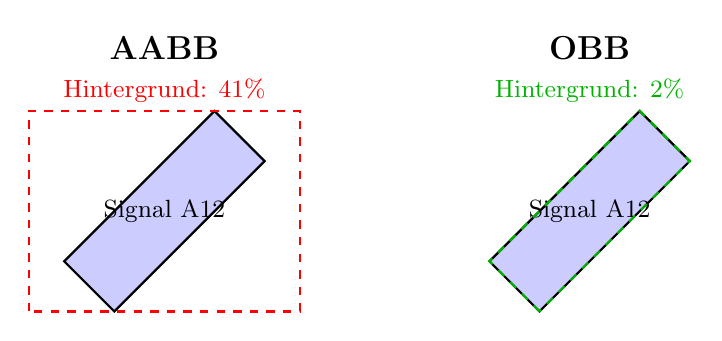
\begin{tikzpicture}[scale=0.9]
    % LEFT: AABB
    \begin{scope}
        \node[above, font=\large\bfseries] at (2, 3.5) {AABB};
        
        % Rotated text at 45 degrees
        \begin{scope}[rotate around={45:(2,1.5)}]
            \draw[thick, fill=blue!20] (0.5,1) rectangle (3.5,2);
            \node[font=\small] at (2,1.5) {Signal A12};
        \end{scope}
        
        % AABB box (red, axis-aligned)
        \draw[thick, red, dashed] (0.086,0.086) rectangle (3.914,2.914);
        
        % Annotations
        \node[below, red, font=\small] at (2, 3.5) {Hintergrund: 41\%};
    \end{scope}
    
    % RIGHT: OBB
    \begin{scope}[xshift=6cm]
        \node[above, font=\large\bfseries] at (2, 3.5) {OBB};
        
        % Rotated text at 45 degrees
        \begin{scope}[rotate around={45:(2,1.5)}]
            \draw[thick, fill=blue!20] (0.5,1) rectangle (3.5,2);
            \node[font=\small] at (2,1.5) {Signal A12};
        \end{scope}
        
        % OBB box (green, rotated with object)
        \begin{scope}[rotate around={45:(2,1.5)}]
            \draw[thick, green!70!black, dashed] (0.5,1) rectangle (3.5,2);
        \end{scope}
        
        % Annotations
        \node[below, green!70!black, font=\small] at (2, 3.5) {Hintergrund: 2\%};
    \end{scope}
\end{tikzpicture}
\caption{AABB vs OBB Vergleich bei rotiertem Textlabel.}
\label{fig:aabb_obb_comparison}
\end{figure}

Dieser hohe Hintergrundanteil hat zwei wesentliche Konsequenzen für die Objekterkennung: Erstens verschlechtert sich das Signal-Rausch-Verhältnis der Eingabedaten für nachgelagerte Verarbeitungsschritte wie OCR\cite{Ma2018ArbitraryOrientedST}. Zweitens steigt die Wahrscheinlichkeit falscher Detektionen, da irrelevante Bildelemente innerhalb der Bounding Box liegen\cite{Ding2019_LearningRoI}.

\subsubsection{Non-Maximum Suppression bei dichten Objektgruppen}

Ein weiteres Problem ergibt sich bei der Nachbearbeitung von Detektionen mittels Non-Maximum Suppression (NMS)\cite{Ren2015_FasterRCNN}. NMS eliminiert redundante Detektionen durch Unterdrückung überlappender Boxen basierend auf ihrer Intersection over Union (IoU):

\begin{equation}
\text{IoU}(B_1, B_2) = \frac{\text{Area}(B_1 \cap B_2)}{\text{Area}(B_1 \cup B_2)}
\end{equation}

Bei dicht platzierten rotierten Objekten führen AABB zu hohen IoU-Werten, obwohl die Objekte selbst nicht überlappen\cite{Ding2019_LearningRoI}. Dies resultiert in fälschlicher Unterdrückung korrekter Detektionen. Abbildung \ref{fig:nms_problem} demonstriert dieses Fehlverhalten anhand zweier nahe beieinanderliegender Textlabels. Die beiden Textobjekte sind um 30° bzw. -30° rotiert und überlappen sich nicht. Ihre achsenparallelen Bounding Boxes hingegen weisen eine signifikante Überlappung mit IoU = 0.42 auf. Bei einem typischen NMS-Schwellenwert von $\tau = 0.4$\cite{Lin2017_FocalLoss} würde eine der beiden korrekten Detektionen fälschlicherweise unterdrückt. Im Gegensatz dazu berechnet sich die IoU zwischen den orientierten Bounding Boxes korrekt zu 0.0, da die Objekte tatsächlich nicht überlappen.

\begin{figure}[H]
\centering
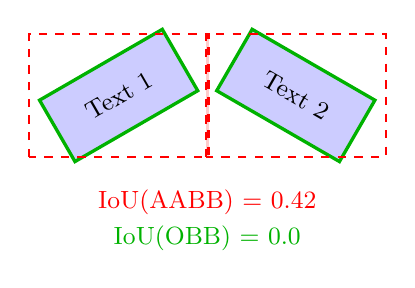
\begin{tikzpicture}[scale=0.9]
    % Two rotated text boxes close together

    % --- Text 1 (30° rotation) ---
    \begin{scope}[rotate around={30:(1.5,2)}]
        \draw[very thick, green!70!black, fill=blue!20] (0.5,1.5) rectangle (2.5,2.5);
        \node[font=\small, rotate=30] at (1.5,2) {Text 1};
    \end{scope}

    % --- Text 2 (-30° rotation) ---
    \begin{scope}[rotate around={-30:(4,2)}]
        \draw[very thick, green!70!black, fill=blue!20] (3,1.5) rectangle (5,2.5);
        \node[font=\small, rotate=-30] at (4,2) {Text 2};
    \end{scope}

    % --- AABBs (red and dashed) ---
    % AABB for Text 1
    \draw[thick, red, dashed] (0.232,1.134) rectangle (2.768,2.866);

    % AABB for Text 2
    \draw[thick, red, dashed] (2.732,1.134) rectangle (5.268,2.866);

    % Overlap region (AABB overlap)
    \fill[red, opacity=0.2] (2.732,1.134) rectangle (2.768,2.866);

    % Annotation
    \node[below, red, font=\small] at (2.75, 0.8) {IoU(AABB) = 0.42};
    \node[below, green!70!black, font=\small] at (2.75, 0.3) {IoU(OBB) = 0.0};
\end{tikzpicture}
\caption{NMS-Problem bei dicht platzierten rotierten Objekten.}
\label{fig:nms_problem}
\end{figure}

\subsection{Oriented Bounding Boxes als Lösung}
\label{sec:orientedboundingboxesalslösung}
Oriented Bounding Boxes erweitern die AABB-Repräsentation um einen zusätzlichen Freiheitsgrad: den Rotationswinkel $\theta$. Eine OBB wird durch fünf Parameter definiert:

\begin{equation}
\text{OBB} = (c_x, c_y, w, h, \theta)
\end{equation}

wobei $(c_x, c_y)$ das Zentrum, $w$ und $h$ die Dimensionen entlang der lokalen Achsen und $\theta \in [-90^\circ, 90^\circ)$ den Rotationswinkel relativ zur horizontalen Bildachse beschreiben. Diese Repräsentation ermöglicht eine eng anliegende Umhüllung rotierter Objekte und reduziert den Hintergrundanteil auf das geometrische Minimum.

\subsubsection{Vorteile für rotierte Objekte}

Die präzisere geometrische Modellierung durch OBB bietet mehrere Vorteile. Bei perfekter Ausrichtung der OBB mit dem Objekt minimiert sich der Hintergrundanteil, während AABB bei starker Rotation erhebliche Hintergrundbereiche umschließen. Die IoU zwischen OBB reflektiert die tatsächliche Objektüberlappung, wodurch Fehlunterdrückungen bei NMS vermieden werden. Dies ist besonders wichtig bei dicht gruppierten Objekten, wo AABB fälschlicherweise hohe Überlappungen anzeigen würden. Zudem kodiert der Parameter $\theta$ explizit die Objektorientierung, was für nachgelagerte Prozesse wie orientierungsabhängige OCR wertvoll ist. Für die Domäne der Gleisplan-Analyse sind diese Eigenschaften besonders relevant, da Symbole entlang der Gleisachsen in beliebigen Winkeln angeordnet sind und oft dicht gruppiert auftreten.

\subsection{Herausforderungen bei der Verwendung von OBB}

Trotz der geometrischen Vorteile bringen OBB zusätzliche Komplexität in die Detektionspipeline, die sich auf Training, Inferenz und Nachbearbeitung auswirkt. Abbildung \ref{fig:obb_challenges} fasst die drei Hauptherausforderungen zusammen: erhöhte Berechnungskomplexität bei der IoU-Berechnung, die Periodizität des Rotationswinkels, die zu Trainingsinstabilität führt, und der erhöhte Trainingsaufwand gegenüber AABB-Modellen.

\begin{figure}[H]
\centering
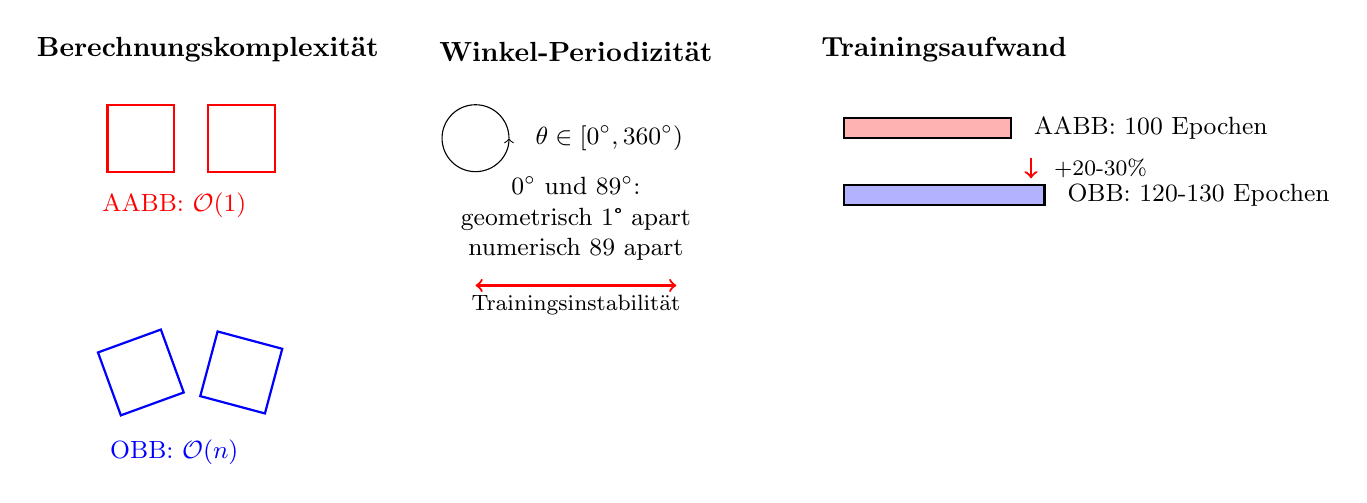
\begin{tikzpicture}[scale=0.85, every node/.style={font=\small}]
    % Challenge 1: Computational Complexity
    \begin{scope}
        \node[above, font=\bfseries] at (2, 3.5) {Berechnungskomplexität};
        
        % AABB: Simple rectangles
        \draw[thick, red] (0.5, 2) rectangle (1.5, 3);
        \draw[thick, red] (2, 2) rectangle (3, 3);
        \node at (1.5, 1.5) {\textcolor{red}{AABB: $\mathcal{O}(1)$}};
        
        % OBB: Rotated rectangles with intersection
        \begin{scope}[shift={(0,-1.5)}]
            \begin{scope}[rotate around={20:(1,0.5)}]
                \draw[thick, blue] (0.5, 0) rectangle (1.5, 1);
            \end{scope}
            \begin{scope}[rotate around={-15:(2.5,0.5)}]
                \draw[thick, blue] (2, 0) rectangle (3, 1);
            \end{scope}
            \node at (1.5, -0.7) {\textcolor{blue}{OBB: $\mathcal{O}(n)$}};
        \end{scope}
    \end{scope}
    
    % Challenge 2: Angle Periodicity
    \begin{scope}[xshift=5.5cm]
        \node[above, font=\bfseries] at (2, 3.5) {Winkel-Periodizität};
        
        % Angle representation
        \draw[->] (1, 2.5) arc (0:360:0.5);
        \node at (2.5, 2.5) {$\theta \in [0^\circ, 360^\circ)$};
        
        % Problem illustration
        \node[align=center] at (2, 1.3) {$0^\circ$ und $89^\circ$:\\geometrisch 1° apart\\numerisch 89 apart};
        
        \draw[thick, red, <->] (0.5, 0.3) -- (3.5, 0.3);
        \node[below, font=\footnotesize] at (2, 0.3) {Trainingsinstabilität};
    \end{scope}
    
    % Challenge 3: Training Overhead
    \begin{scope}[xshift=11cm]
        \node[above, font=\bfseries] at (2, 3.5) {Trainingsaufwand};
        
        % Training progress bars
        \draw[thick, fill=red!30] (0.5, 2.5) rectangle (3, 2.8);
        \node[right] at (3.2, 2.65) {AABB: 100 Epochen};
        
        \draw[thick, fill=blue!30] (0.5, 1.5) rectangle (3.5, 1.8);
        \node[right] at (3.7, 1.65) {OBB: 120-130 Epochen};
        
        % Arrow indicating increase
        \draw[thick, red, ->] (3.3, 2.2) -- (3.3, 1.9);
        \node[right, font=\footnotesize] at (3.5, 2.05) {+20-30\%};
    \end{scope}
\end{tikzpicture}
\caption{Hauptherausforderungen bei OBB-Verwendung.}
\label{fig:obb_challenges}
\end{figure}

\subsubsection{Erhöhte Berechnungskomplexität}

Die Berechnung der Intersection over Union zwischen zwei OBB ist algorithmisch aufwendiger als bei AABB. Während die AABB-IoU durch einfache Min-Max-Operationen in konstanter Zeit $\mathcal{O}(1)$ berechnet werden kann, erfordert die OBB-IoU die Lösung eines Polygon-Clipping-Problems\cite{Zhou2017EastAE}:

\begin{equation}
\text{IoU}_{\text{OBB}}(B_1, B_2) = \frac{\text{Area}(P_1 \cap P_2)}{\text{Area}(P_1 \cup P_2)}
\end{equation}

wobei $P_1$ und $P_2$ die als Vierecke repräsentierten OBB sind. Die Schnittpunktberechnung zwischen den Kantensegmenten skaliert mit $\mathcal{O}(n^2)$ für $n$-Ecke, was in der Praxis zu einem Faktor 3-5 langsameren NMS-Durchläufen führt\cite{Xie2021OrientedRD}.

\subsubsection{Winkel-Periodizität und Trainingsinstabilität}

Der Rotationswinkel $\theta$ weist eine zyklische Periodizität auf: Eine Rotation um 180° (bzw. bei symmetrischen Objekten um 90°) resultiert in einer geometrisch identischen Bounding Box\cite{Yang2021RSDETR,Zhao2023ABFL}. Dies führt zu Ambiguitäten in der Netzwerk-Ausgabe. Betrachtet man beispielsweise zwei Vorhersagen $\theta_1 = 0^\circ$ und $\theta_2 = 89^\circ$ für dasselbe Objekt, so sind diese geometrisch nur 1° voneinander entfernt, numerisch jedoch 89 Einheiten. Standard-Regressionsverluste (z.B. Smooth L1) behandeln diese Diskrepanz linear, was zu instabilen Gradienten führt.


\subsubsection{Erhöhter Trainingsaufwand}

Die zusätzliche Parameterregression für $\theta$ erhöht die Komplexität des Lernproblems. Empirische Studien zeigen, dass OBB-Modelle typischerweise 20-30\% mehr Trainingsepochen benötigen als vergleichbare AABB-Modelle, um ähnliche Konvergenzniveaus zu erreichen\cite{Xie2021OrientedRD}. Dies resultiert aus der Notwendigkeit, sowohl die präzise Lokalisierung als auch die korrekte Orientierungsprädiktion zu erlernen.

\subsection{YOLOv8-OBB Architektur}

YOLOv8 bietet eine spezialisierte OBB-Variante, die für die Symbolerkennung geeignet ist. Die Architekturwahl wird in Kapitel~\ref{chap:konzeption} begründet. YOLOv8-OBB erweitert die Standard-Architektur um die Regression des Rotationsparameters $\theta$, während die grundlegende Netzwerkstruktur aus Backbone, Neck und Detection Heads erhalten bleibt\cite{yolov8_ultralytics}. Die schematische Architektur ist in Abbildung \ref{fig:yolov8_architecture} dargestellt und zeigt den Informationsfluss vom Eingabebild über die Feature-Extraktion bis zu den finalen OBB-Vorhersagen. Der Backbone extrahiert hierarchische Merkmale auf fünf Auflösungsstufen, das Neck fusioniert diese über Skalen hinweg, und die drei spezialisierten Detection Heads produzieren Vorhersagen für kleine, mittlere und große Objekte.

\begin{figure}[H]
\centering
\hspace*{1.5cm} 
\begin{tikzpicture}[
    scale=0.9,
    node distance=1.2cm and 0.5cm,
    module/.style={
        rectangle, 
        draw, 
        minimum width=3.2cm, 
        minimum height=1cm, 
        align=center, 
        fill=blue!10,
        font=\small
    },
    arrow/.style={->, >=stealth, thick, rounded corners}
]

    % 1. Input
    \node[module, fill=gray!20] (input) {Input\\$1024 \times 1024 \times 3$};
    
    % 2. Backbone
    \node[module, below=of input, fill=blue!20] (backbone) {CSPNet Backbone\\(C2f Modules)};
    
    % 3. Multi-scale features
    \node[module, below=of backbone, fill=green!20, minimum width=8cm] (features) {Multi-Scale Features\\(P3, P4, P5)};
    
    % 4. Neck
    \node[module, below=of features, fill=orange!20] (neck) {PANet Neck\\(FPN + PAN)};
    
    % 5. Detection heads
    \node[module, below=1.5cm of neck, fill=red!20, minimum width=2.8cm] (head2) {Head P4\\(Medium)};
    \node[module, left=0.2cm of head2, fill=red!20, minimum width=2.8cm] (head1) {Head P3\\(Small)};
    \node[module, right=0.2cm of head2, fill=red!20, minimum width=2.8cm] (head3) {Head P5\\(Large)};
    
    % 6. Outputs
    \node[module, below=1.2cm of head2, fill=purple!20, minimum width=8cm] (output) {OBB Predictions\\$(c_x, c_y, w, h, \theta, \text{cls})$};
    
    % Arrows
    \draw[arrow] (input) -- (backbone);
    \draw[arrow] (backbone) -- (features);
    \draw[arrow] (features) -- (neck);
    
    \draw[arrow] (neck.south) -- (head2.north); 
    \draw[arrow] (neck.south) -| (head1.north); 
    \draw[arrow] (neck.south) -| (head3.north); 
    
    \draw[arrow] (head2.south) -- (output.north);
    \draw[arrow] (head1.south) -- (head1.south |- output.north); 
    \draw[arrow] (head3.south) -- (head3.south |- output.north); 
    
    % Annotations
    \node[right=0.8cm of backbone, font=\footnotesize, align=left] {
        \textbf{Feature Extraction:}\\
        5 Resolution Levels
    };
    
    \node[right=0.8cm of neck, font=\footnotesize, align=left] {
        \textbf{Feature Fusion:}\\
        Top-Down + Bottom-Up
    };
    
    \node[right=0.2cm of head3, font=\footnotesize, align=left, text width=3.5cm] {
        \textbf{Decoupled Heads:}\\
        Separate Classification\\
        \& Regression
    };

\end{tikzpicture}
\caption{YOLOv8-OBB Architektur.}
\label{fig:yolov8_architecture}
\end{figure}

\subsubsection{Netzwerkkomponenten}

Die Architektur gliedert sich in drei funktionale Blöcke. Der Backbone extrahiert hierarchische Merkmale aus den Eingabebildern und verwendet eine auf CSPNet basierende Architektur mit Cross Stage Partial Connections\cite{Wang2020_CSPNet}. Die sogenannten C2f-Module (CSP Bottleneck with 2 Convolutions, faster) ersetzen die C3-Module früherer Versionen und bieten eine effizientere Gradientenfluss-Charakteristik bei gleichzeitiger Reduktion der Parameteranzahl. Das Neck-Modul fusioniert Merkmale unterschiedlicher Auflösungsstufen durch eine Kombination aus Top-Down- und Bottom-Up-Pfaden. Die Path Aggregation Network (PANet) Architektur\cite{Liu2018_PANet} ermöglicht eine effektive Informationspropagation zwischen den Skalen, was für die Detektion sowohl kleiner als auch großer Objekte essentiell ist. YOLOv8 folgt einem Anchor-Free-Ansatz\cite{Tian2019FCOS}, bei dem Objektzentren direkt vorhergesagt werden, anstatt vordefinierte Anker-Boxen zu verwenden. Die Heads sind dezentralisiert (decoupled): Separate Zweige regredieren die Lokalisierung (inklusive $\theta$) und die Klassifikation. Diese Entkopplung verbessert die Konvergenz, da die beiden Aufgaben unterschiedliche Repräsentationen erfordern\cite{Ge2021_YOLOX}.

\subsubsection{Verlustfunktion und Training}

Das Training von YOLOv8-OBB optimiert eine kombinierte Verlustfunktion, die drei Komponenten umfasst:

\begin{equation}
\mathcal{L}_{\text{total}} = \lambda_{\text{box}} \mathcal{L}_{\text{box}} + \lambda_{\text{cls}} \mathcal{L}_{\text{cls}} + \lambda_{\text{dfl}} \mathcal{L}_{\text{dfl}}
\end{equation}

Die Box-Loss $\mathcal{L}_{\text{box}}$ quantifiziert die Lokalisierungsgenauigkeit der vorhergesagten OBB gegenüber der Ground Truth. Die Classification-Loss $\mathcal{L}_{\text{cls}}$ verwendet Binary Cross-Entropy für die Klassenzuordnung\cite{Lin2017_FocalLoss}. Die Distribution Focal Loss (DFL)\cite{Li2020GeneralizedFocal} verbessert die Bounding-Box-Regression durch Modellierung der Koordinaten als Verteilungen anstelle von Punktschätzungen.

Die konkreten Trainingsparameter und -ergebnisse für den im Rahmen dieser Arbeit trainierten Detektor werden in Kapitel 6 detailliert dokumentiert. Die Kombination aus Echtzeitfähigkeit, Rotationsinvarianz und Anchor-Free-Design macht YOLOv8-OBB zu einem geeigneten Kandidaten für die Gleisplananalyse. Die endgültige Architekturentscheidung 
wird in Kapitel~\ref{chap:konzeption} dokumentiert.

\subsection{Relevanz für Gleisplan-Analyse}

Die beschriebenen OBB-Eigenschaften sind besonders relevant für die automatisierte Analyse von Gleisplänen. Technische Zeichnungen dieses Typs weisen drei charakteristische Merkmale auf, die den Einsatz orientierter Bounding Boxes notwendig machen. Symbole folgen der Topologie der Gleisachsen und können daher in jedem Winkel $\theta \in [0^\circ, 360^\circ)$ vorliegen. In Bahnhöfen und Weichenstraßen treten Symbole räumlich konzentriert auf, wobei AABB-basierte NMS zu Fehlunterdrückungen führen würde. Die vom OBB-Detektor gelieferte Rotation $\theta$ ist für nachgelagerte Prozesse wie die orientierungsabhängige OCR (vgl. Kapitel 6.3) essentiell, da Textlabels entsprechend ihrer Ausrichtung verarbeitet werden müssen.

Die in Kapitel 4 definierten funktionalen Anforderungen an die Symbolerkennung erfordern daher zwingend den Einsatz rotationsinvarianter Detektionsverfahren. Die in Kapitel 6 beschriebene Implementierung nutzt YOLOv8-OBB mit Standard-Konfiguration für die Detektion von 13 domänenspezifischen Symbolklassen (vgl. Tabelle \ref{tab:symbole} in Kapitel 4).

\section{Optical Character Recognition (OCR)}
\label{sec:ocr}

Die optische Zeichenerkennung bildet das verbindende Element zwischen der visuellen Symbolerkennung und der semantischen Interpretation von Gleisplänen. Während die in Abschnitt \ref{sec:objekterkennung} beschriebene Objekterkennung Symbole lokalisiert und klassifiziert, liefert sie zunächst keine Information über die zugehörigen Textinhalte. Erst durch die zuverlässige Extraktion von Signalbezeichnungen (z.\,B. \enquote{AS102}), Kilometerangaben (z.\,B. \enquote{18.1606}) und Balisen-Kennungen (z.\,B. \enquote{1234}) erhalten die erkannten Symbole ihre vollständige technische Bedeutung.

Dieser Abschnitt behandelt zunächst die allgemeinen Grundlagen der optischen Zeichenerkennung, bevor die spezifischen Herausforderungen technischer Zeichnungen und die für Gleispläne relevanten Lösungsansätze dargelegt werden. Die Progression folgt dabei dem Muster der vorangegangenen Abschnitte: vom allgemeinen Prinzip über moderne Architekturen bis zur domänenspezifischen Anwendung.

\subsection{Grundlagen und Entwicklung der OCR-Technologie}
\label{subsec:ocr_grundlagen}

Die optische Zeichenerkennung bezeichnet die automatisierte Umwandlung von Bildern, die Text enthalten, in maschinenlesbaren Text. Diese Aufgabe lässt sich konzeptionell in eine Verarbeitungskette unterteilen, die in Abbildung \ref{fig:ocr_pipeline_konzept} dargestellt ist.

\begin{figure}[h]
\centering
\begin{tikzpicture}[
    % Größerer vertikaler Abstand (2.5cm) für die Labels dazwischen
    node distance=2.5cm and 1.0cm,
    box/.style={
        rectangle, 
        draw, 
        thick, 
        minimum width=3.2cm, % Etwas breiter für besseren Textumbruch
        minimum height=1cm, 
        align=center, 
        font=\small, 
        rounded corners=2pt
    },
    arrow/.style={->, >=stealth, thick, rounded corners},
    annotation/.style={font=\scriptsize, align=center, text=gray!40!black}
]

    % --- ZEILE 1 (Nach Rechts) ---
    
    % 1. Input
    \node[box, fill=blue!10] (input) {Eingabebild\\(Dokument/Scan)};
    
    % 2. Vorverarbeitung
    \node[box, right=of input, fill=yellow!20] (preproc) {Vorverarbeitung\\(Binarisierung)};
    \node[annotation, below=0.1cm of preproc] {Kontrast,\\Rauschen};
    
    % 3. Textdetektion
    \node[box, right=of preproc, fill=orange!20] (detect) {Textdetektion\\(Lokalisierung)};
    \node[annotation, below=0.1cm of detect] {Bounding\\Boxes};

    
    % --- ZEILE 2 (Nach Links, unter der ersten Zeile) ---
    
    % 4. Zeichenerkennung (Unter Detektion)
    \node[box, below=of detect, fill=green!20] (recog) {Zeichenerkennung\\(Recognition)};
    \node[annotation, below=0.1cm of recog] {CNN/LSTM\\Decoder};
    
    % 5. Nachverarbeitung (Links von Erkennung)
    \node[box, left=of recog, fill=purple!20] (post) {Nachverarbeitung\\(Validierung)};
    \node[annotation, below=0.1cm of post] {Regex,\\Korrektur};
    
    % 6. Ausgabe (Links von Post)
    \node[box, left=of post, fill=gray!10] (output) {Ausgabetext\\(String)};
    

    % --- PFEILE ---
    \draw[arrow] (input) -- (preproc);
    \draw[arrow] (preproc) -- (detect);
    
    % Der Pfeil von Zeile 1 zu Zeile 2 (Rechts außen runter)
    \draw[arrow] (detect.south) -- (recog.north);
    
    % Pfeile zurück nach links
    \draw[arrow] (recog) -- (post);
    \draw[arrow] (post) -- (output);

\end{tikzpicture}
\caption{Konzeptionelle OCR-Pipeline (Zweizeilige Darstellung)}
\label{fig:ocr_pipeline_konzept}
\end{figure}
Die \textbf{Vorverarbeitung} bereitet das Eingabebild für die nachfolgenden Schritte auf. Typische Operationen umfassen Kontrastverbesserung, Rauschunterdrückung und Binarisierung (Umwandlung in Schwarz-Weiß). Bei technischen Zeichnungen ist zusätzlich die Entfernung störender Linienelemente relevant \cite{Tombre}.

Die \textbf{Textdetektion} lokalisiert Bereiche im Bild, die Text enthalten. Moderne Verfahren verwenden neuronale Netze zur Segmentierung von Textregionen, wobei die Ausgabe typischerweise als Bounding Boxes oder Polygone erfolgt \cite{liao2019realtimescenetextdetection}.

Die \textbf{Zeichenerkennung} wandelt die lokalisierten Bildausschnitte in Zeichenfolgen um. Dies ist die eigentliche \enquote{Erkennung} im engeren Sinne und bildet den rechenintensivsten Schritt der Pipeline.

Die \textbf{Nachverarbeitung} validiert und korrigiert die erkannten Texte. Für domänenspezifische Anwendungen wie Gleispläne können hier Musterprüfungen (Regular Expressions) und Plausibilitätskontrollen integriert werden.

\subsubsection{Historische Entwicklung}

Die Entwicklung der OCR-Technologie lässt sich in drei Phasen unterteilen, die in Tabelle \ref{tab:ocr_evolution} zusammengefasst sind.

\begin{table}[H]
\centering
\renewcommand{\arraystretch}{1.3}
\begin{tabular}{|p{2.5cm}|p{3cm}|p{4cm}|p{4cm}|}
\hline
\textbf{Phase} & \textbf{Zeitraum} & \textbf{Methodik} & \textbf{Limitierungen} \\
\hline
Regelbasiert & 1950--1980 & Template Matching, Merkmalsdeskriptoren & Nur monospace-Schriften, keine Variabilität \\
\hline
Statistisch & 1980--2010 & Hidden Markov Models (HMM), SVM mit HOG-Features & Manuelles Feature-Engineering, begrenzte Robustheit \\
\hline
Deep Learning & 2010--heute & CNN + RNN, Transformer, End-to-End-Training & Hoher Datenbedarf, Rechenaufwand \\
\hline
\end{tabular}
\caption{Evolution der OCR-Technologie über drei methodische Phasen\cite{Mori1999}}
\label{tab:ocr_evolution}
\end{table}

Die erste Generation basierte auf expliziten Mustervergleichen: Für jedes zu erkennende Zeichen wurde ein Template definiert, das pixelweise mit dem Eingabebild verglichen wurde \cite{Mori1999}. Diese Ansätze funktionierten nur bei exakt passenden Schriftarten und -größen.

Die zweite Generation führte statistische Modelle ein. Hidden Markov Models (HMM) modellierten die sequenzielle Struktur von Text, während Support Vector Machines (SVM) auf manuell konstruierten Merkmalen (z.\,B. Histogram of Oriented Gradients) operierten \cite{Smith2007}. Diese Verfahren ermöglichten erstmals Robustheit gegenüber moderaten Variationen, erforderten jedoch aufwendiges Feature-Engineering.

Die dritte Generation nutzt Deep Learning für End-to-End-Erkennung. Convolutional Neural Networks (CNN) extrahieren visuelle Merkmale automatisch aus Trainingsbeispielen, während Recurrent Neural Networks (RNN) die sequenzielle Abhängigkeit zwischen Zeichen modellieren \cite{Shi2017_CRNN}. Diese Kombination ermöglicht die Erkennung beliebiger Schriftarten und -stile ohne manuelle Merkmalsdefiniton.

\subsection{Architekturen moderner OCR-Systeme}
\label{subsec:ocr_architekturen}

Moderne OCR-Systeme basieren auf zwei dominierenden Architekturparadigmen: der CRNN-Architektur (Convolutional Recurrent Neural Network) und Transformer-basierten Ansätzen. Beide werden im Folgenden erläutert.

\subsubsection{CRNN-Architektur}

Die CRNN-Architektur, eingeführt von Shi et al. \cite{Shi2017_CRNN}, kombiniert drei Komponenten zu einem End-to-End-trainierbaren System (Abbildung \ref{fig:crnn_architecture}).

\begin{figure}[H]
\centering
\begin{tikzpicture}[
    scale=0.8,
    node distance=1.0cm and 0.8cm,
    layer/.style={rectangle, draw, thick, minimum width=2.2cm, minimum height=0.9cm, align=center, font=\small},
    arrow/.style={->, >=stealth, thick}
]
    % Input
    \node[layer, fill=gray!20] (input) {Bildausschnitt\\$W \times H \times 1$};
    
    % CNN Layers
    \node[layer, below=of input, fill=blue!20] (cnn1) {Conv + Pool\\$\times 4$};
    \node[layer, below=of cnn1, fill=blue!30] (cnn2) {Feature Maps\\$\frac{W}{4} \times 1 \times 512$};
    
    % Reshape
    \node[layer, below=of cnn2, fill=yellow!30] (reshape) {Reshape\\Sequenz von $T$ Vektoren};
    
    % BiLSTM
    \node[layer, below=of reshape, fill=orange!30] (lstm) {BiLSTM\\2 Schichten, 256 Hidden};
    
    % CTC
    \node[layer, below=of lstm, fill=green!30] (ctc) {CTC-Decoder\\Alignment + Deduplizierung};
    
    % Output
    \node[layer, below=of ctc, fill=purple!20] (output) {Ausgabetext\\z.\,B. \enquote{AS102}};
    
    % Arrows
    \draw[arrow] (input) -- (cnn1);
    \draw[arrow] (cnn1) -- (cnn2);
    \draw[arrow] (cnn2) -- (reshape);
    \draw[arrow] (reshape) -- (lstm);
    \draw[arrow] (lstm) -- (ctc);
    \draw[arrow] (ctc) -- (output);
    
    % Side labels
    \node[right=0.5cm of cnn1, font=\scriptsize, align=left] {Visuelle\\Merkmale};
    \node[right=0.5cm of lstm, font=\scriptsize, align=left] {Sequenzielle\\Abhängigkeiten};
    \node[right=0.5cm of ctc, font=\scriptsize, align=left] {Variable\\Längen};
    
    % Component brackets
    \draw[decorate, decoration={brace, amplitude=5pt}, thick] 
        ([xshift=-0.3cm]cnn1.north west) -- ([xshift=-0.3cm]cnn2.south west) 
        node[midway, left=8pt, font=\small\bfseries] {CNN};
    \draw[decorate, decoration={brace, amplitude=5pt}, thick] 
        ([xshift=-0.3cm]lstm.north west) -- ([xshift=-0.3cm]lstm.south west) 
        node[midway, left=8pt, font=\small\bfseries] {RNN};
    \draw[decorate, decoration={brace, amplitude=5pt}, thick] 
        ([xshift=-0.3cm]ctc.north west) -- ([xshift=-0.3cm]ctc.south west) 
        node[midway, left=8pt, font=\small\bfseries] {CTC};
\end{tikzpicture}
\caption{CRNN-Architektur}
\label{fig:crnn_architecture}
\end{figure}

\textbf{CNN-Komponente (Feature Extraction):} Ein Convolutional Neural Network extrahiert visuelle Merkmale aus dem Eingabebild. Durch sukzessive Faltungs- und Pooling-Operationen wird das Bild auf eine Sequenz von Merkmalsvektoren reduziert. Ein Bildausschnitt der Größe $W \times H$ wird typischerweise auf $T = W/4$ Zeitschritte mit je 512 Merkmalskanälen komprimiert\cite{Shi2017_CRNN}.

\textbf{RNN-Komponente (Sequence Modeling):} Ein bidirektionales LSTM (Long Short-Term Memory) \cite{Hochreiter1997_LSTM} verarbeitet die Merkmalssequenz und modelliert kontextuelle Abhängigkeiten zwischen benachbarten Zeichen. Die Bidirektionalität ermöglicht die Berücksichtigung sowohl vergangener als auch zukünftiger Kontextinformation.

\textbf{CTC-Decoder (Transcription):} Die Connectionist Temporal Classification (CTC) \cite{Graves2006_CTC} löst das Problem variabler Ausgabelängen. Da die Anzahl der CNN-Ausgabespalten nicht mit der Anzahl der Textzeichen übereinstimmt, führt CTC ein \enquote{Blank}-Symbol ein und definiert eine Verlustfunktion, die alle möglichen Alignments zwischen Eingabe und Ausgabe marginalisiert:

\begin{equation}
P(y \mid x) = \sum_{\pi \in \mathcal{B}^{-1}(y)} \prod_{t=1}^{T} P(\pi_t \mid x)
\label{eq:ctc_loss}
\end{equation}

wobei $y$ die Zielsequenz, $x$ die Eingabe, $\mathcal{B}^{-1}(y)$ die Menge aller Pfade bezeichnet, die nach Entfernung von Blanks und Deduplizierung $y$ ergeben, und $P(\pi_t \mid x)$ die Wahrscheinlichkeit des Symbols $\pi_t$ zum Zeitpunkt $t$ ist.

Für Maschinenbau-Ingenieure lässt sich die CTC-Funktionsweise anschaulich erklären: Das Netz gibt für jeden Zeitschritt (jede Spalte des Bildes) eine Wahrscheinlichkeitsverteilung über alle möglichen Zeichen aus. Die Ausgabe \enquote{A--S-11-0-2} (wobei \enquote{-} das Blank-Symbol bezeichnet) wird durch Entfernung der Blanks und Zusammenfassung aufeinanderfolgender identischer Zeichen zu \enquote{AS102} dekodiert.

\subsubsection{Transformer-basierte OCR}

Neuere Ansätze ersetzen die RNN-Komponente durch Transformer-Architekturen \cite{Vaswani2017_Attention}. Der TrOCR-Ansatz \cite{li2022trocrtransformerbasedopticalcharacter} verwendet einen Vision Transformer (ViT) als Encoder und einen Text Transformer als Decoder. Vision Transformer ist ein Transformer Modell, das Bilder als Sequenz von Patches verarbeitet\cite{Dosovitskiy2021_ViT} Der zentrale Mechanismus ist die Self-Attention:

\begin{equation}
\text{Attention}(Q, K, V) = \text{softmax}\left(\frac{QK^T}{\sqrt{d_k}}\right) V
\label{eq:attention}
\end{equation}

wobei $Q$ (Query), $K$ (Key) und $V$ (Value) lineare Projektionen der Eingabe sind und $d_k$ die Dimensionalität der Keys bezeichnet. Die Division durch $\sqrt{d_k}$ stabilisiert die Gradienten.

Transformer-basierte Ansätze bieten Vorteile bei langen Sequenzen und ermöglichen effizientere Parallelisierung während des Trainings. Für kurze Texte wie Signalbezeichnungen (typischerweise 3--8 Zeichen) sind die Vorteile jedoch marginal, weshalb CRNN-basierte Systeme wie PaddleOCR in der Praxis häufig bevorzugt werden.

\subsubsection{Vergleich der Architekturen}

Tabelle \ref{tab:ocr_arch_comparison} fasst die wesentlichen Unterschiede zwischen CRNN und Transformer-basierten Ansätzen zusammen.
\begin{table}[H]
\centering
\renewcommand{\arraystretch}{1.3}
\begin{tabular}{|p{3.5cm}|p{5cm}|p{5cm}|}
\hline
\textbf{Kriterium} & \textbf{CRNN (z.\,B. PaddleOCR)} & \textbf{Transformer (z.\,B. TrOCR)} \\
\hline
Genauigkeit (kurze Texte) & >95\% \cite{du2020ppocrpracticalultralightweight} & >95\% \cite{li2022trocrtransformerbasedopticalcharacter} \\
\hline
Inferenzzeit (CPU) & 8--15 ms/Bild \cite{du2020ppocrpracticalultralightweight} & 50--150 ms/Bild\footnotemark \\
\hline
Modellgröße & 8--12 MB \cite{du2020ppocrpracticalultralightweight} & 300--500 MB \cite{li2022trocrtransformerbasedopticalcharacter} \\
\hline
Trainingsdatenbedarf & Moderat (10k--100k Samples) & Hoch (>1M Samples für Pretraining) \cite{li2022trocrtransformerbasedopticalcharacter} \\
\hline
\end{tabular}
\caption{Vergleich von CRNN- und Transformer-basierten OCR-Architekturen}
\label{tab:ocr_arch_comparison}
\end{table}
\footnotetext{Transformer-basierte Modelle erfordern aufgrund des quadratischen 
Attention-Mechanismus höhere Inferenzzeiten \cite{Vaswani2017_Attention}.}

\subsection{OCR-Systeme im praktischen Einsatz}
\label{subsec:ocr_systeme}

Für die praktische Anwendung stehen mehrere etablierte OCR-Frameworks zur Verfügung, die unterschiedliche Stärken aufweisen.

\subsubsection{Tesseract}

Tesseract \cite{Smith2007} ist eine Open-Source-Engine, die ursprünglich von Hewlett-Packard entwickelt und später von Google weiterentwickelt wurde. Seit Version 4.0 verwendet Tesseract ein LSTM-basiertes Erkennungsmodell. Die Konfiguration erfolgt über Page Segmentation Modes (PSM), die das erwartete Dokumentlayout spezifizieren:

\begin{itemize}
    \item \textbf{PSM 7}: Einzelne Textzeile -- optimal für isolierte Beschriftungen
    \item \textbf{PSM 8}: Einzelnes Wort -- für kompakte Labels
    \item \textbf{PSM 13}: Raw Line -- für einzelne Textzeilen ohne Layoutsegmentierung, optimal für isolierte Beschriftungen
\end{itemize}

Eine Whitelist-Funktionalität ermöglicht die Einschränkung des Zeichensatzes auf erwartete Zeichen (z.\,B. nur Großbuchstaben und Ziffern für Signalbezeichnungen), was die Erkennungsgenauigkeit in domänenspezifischen Anwendungen erhöht.

\subsubsection{PaddleOCR}

PaddleOCR \cite{du2020ppocrpracticalultralightweight} ist ein vom chinesischen Technologiekonzern Baidu entwickeltes Framework, das eine vollständige Pipeline aus Textdetektion, Winkelklassifikation und Texterkennung bereitstellt. Die PP-OCRv3-Architektur besteht aus drei Komponenten:

\begin{enumerate}
    \item \textbf{DB-Detektor (Differentiable Binarization)}: Lokalisiert Textregionen durch semantische Segmentierung mit differenzierbarer Schwellenwertberechnung \cite{liao2019realtimescenetextdetection}.
    \item \textbf{Winkelklassifikator}: Bestimmt die Orientierung des Textes (0° oder 180°) zur automatischen Korrektur.
    \item \textbf{CRNN-Recognizer}: Erkennt die Zeichenfolge basierend auf der in Abschnitt \ref{subsec:ocr_architekturen} beschriebenen Architektur.
\end{enumerate}

\begin{figure}[H]
\centering
\begin{tikzpicture}[
    scale=0.85,
    node distance=1.5cm,
    box/.style={rectangle, draw, thick, minimum width=3cm, minimum height=1cm, align=center, font=\small, rounded corners=2pt},
    arrow/.style={->, >=stealth, thick}
]
    % Input
    \node[box, fill=gray!20] (input) {Eingabebild};
    
    % Detection
    \node[box, below=of input, fill=blue!20] (detect) {DB-Detektor\\(Texterkennung)};
    
    % Crop
    \node[box, below=of detect, fill=yellow!20] (crop) {ROI-Extraktion\\(Bildausschnitte)};
    
    % Angle
    \node[box, below left=1cm and 0.5cm of crop, fill=orange!20] (angle) {Winkel-\\Klassifikator};
    
    % Recognition
    \node[box, below right=1cm and 0.5cm of crop, fill=green!20] (recog) {CRNN-\\Recognizer};
    
    % Output
    \node[box, below=2.5cm of crop, fill=purple!20] (output) {Erkannte Texte\\+ Positionen};
    
    % Arrows
    \draw[arrow] (input) -- (detect);
    \draw[arrow] (detect) -- (crop);
    \draw[arrow] (crop) -| (angle);
    \draw[arrow] (crop) -| (recog);
    \draw[arrow] (angle) |- (output);
    \draw[arrow] (recog) |- (output);
    
    % Annotations
    \node[right=0.3cm of detect, font=\scriptsize, align=left] {Polygone/Boxes\\für Textregionen};
    \node[left=0.3cm of angle, font=\scriptsize, align=right] {0° oder 180°\\Korrektur};
    \node[right=0.3cm of recog, font=\scriptsize, align=left] {Zeichenfolge\\+ Konfidenz};
\end{tikzpicture}
\caption{PaddleOCR-Pipeline: Dreistufige Architektur mit Detektion, Winkelkorrektur und Erkennung.}
\label{fig:paddleocr_pipeline}
\end{figure}

\subsubsection{Vergleich der OCR-Systeme}

Tabelle \ref{tab:ocr_systems_comparison} vergleicht die für technische Zeichnungen relevanten OCR-Systeme.

\begin{table}[H]
\centering
\small
\renewcommand{\arraystretch}{1.3}
\begin{tabular}{|p{2cm}|p{2.5cm}|p{4.5cm}|p{4.5cm}|}
\hline
\textbf{System} & \textbf{Architektur} & \textbf{Stärken} & \textbf{Schwächen} \\
\hline
Tesseract & LSTM-basiert & Whitelist-Funktion, geringer Ressourcenbedarf & Empfindlich bei Rotation, langsam bei vielen ROIs \\
\hline
PaddleOCR & DB + CRNN & Integrierte Winkelerkennung, schnell, robust & Komplexere Installation, größeres Modell\\
\hline
EasyOCR & CRAFT(Character Region Awareness for Text) + CRNN \cite{baek2019characterregionawarenesstext} & Einfache API, gute Winkeltoleranz & Langsamer, weniger konfigurierbar \\
\hline
TrOCR & Transformer & State-of-the-Art Genauigkeit & Hoher GPU-Bedarf, langsam\\
\hline
\end{tabular}
\caption{Vergleich etablierter OCR-Systeme für technische Anwendungen}
\label{tab:ocr_systems_comparison}
\end{table}
\subsection{Evaluationsmetriken für Texterkennung}
\label{subsec:ocr_metriken}

Analog zu den Evaluationsmetriken für die Objekterkennung (Abschnitt \ref{subsec:evaluationsmetriken}) erfordert die Bewertung von OCR-Systemen standardisierte Metriken, die Erkennungsfehler auf verschiedenen Granularitätsebenen quantifizieren. Diese Metriken basieren auf der Levenshtein-Distanz \cite{levenshtein1966}, welche die minimale Anzahl von Editieroperationen (Einfügungen, Löschungen, Ersetzungen) misst, die erforderlich sind, um eine Zeichenkette in eine andere zu transformieren.

\subsubsection{Character Error Rate}

Die \textbf{Character Error Rate (CER)} ist die fundamentale Metrik zur Bewertung von OCR-Systemen und quantifiziert den Anteil fehlerhafter Zeichen im erkannten Text relativ zur Ground Truth \cite{Rice1996_OCRAccuracy}:

\begin{equation}
\text{CER} = \frac{S + D + I}{N}
\label{eq:cer}
\end{equation}

wobei $S$ die Anzahl der Substitutionen (falsch erkannte Zeichen), $D$ die Anzahl der Deletionen (fehlende Zeichen), $I$ die Anzahl der Insertionen (zusätzlich eingefügte Zeichen) und $N$ die Gesamtanzahl der Zeichen in der Ground Truth bezeichnet. Ein CER-Wert von 0 bedeutet perfekte Erkennung, während Werte über 1 theoretisch möglich sind, wenn die Anzahl der Fehler die Anzahl der Referenzzeichen übersteigt.

Die Berechnung der einzelnen Fehlerkomponenten erfolgt mittels dynamischer Programmierung durch den Wagner-Fischer-Algorithmus \cite{Wagner1974_StringCorrection}, der die optimale Alignment-Sequenz zwischen Ground Truth und OCR-Ausgabe ermittelt.

\begin{figure}[H]
\centering
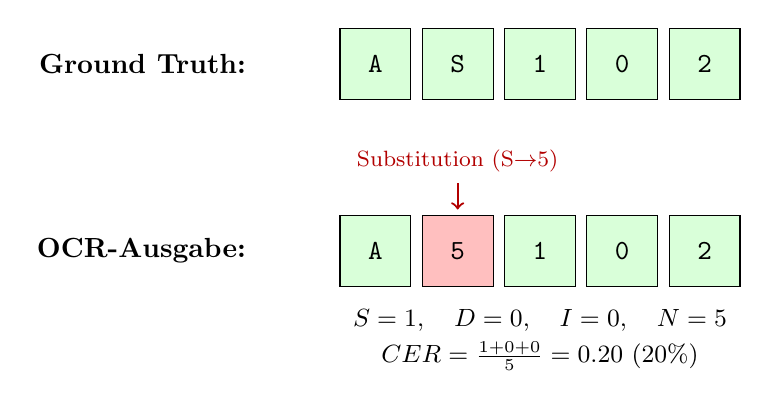
\begin{tikzpicture}[scale=0.95]
    % Ground Truth
    \node[font=\bfseries, anchor=east] at (-0.5, 3) {Ground Truth:};
    \foreach \char [count=\i] in {A,S,1,0,2} {
        \node[draw, minimum width=0.9cm, minimum height=0.9cm, fill=green!15, font=\ttfamily] 
            at (\i*1.1, 3) {\char};
    }
    
    % OCR Output
    \node[font=\bfseries, anchor=east] at (-0.5, 0.5) {OCR-Ausgabe:};
    \node[draw, minimum width=0.9cm, minimum height=0.9cm, fill=green!15, font=\ttfamily] at (1.1, 0.5) {A};
    \node[draw, minimum width=0.9cm, minimum height=0.9cm, fill=red!25, font=\ttfamily] at (2.2, 0.5) {5};
    \node[draw, minimum width=0.9cm, minimum height=0.9cm, fill=green!15, font=\ttfamily] at (3.3, 0.5) {1};
    \node[draw, minimum width=0.9cm, minimum height=0.9cm, fill=green!15, font=\ttfamily] at (4.4, 0.5) {0};
    \node[draw, minimum width=0.9cm, minimum height=0.9cm, fill=green!15, font=\ttfamily] at (5.5, 0.5) {2};
    
    % Error indicator
    \draw[->, thick, red!70!black] (2.2, 1.4) -- (2.2, 1.05);
    \node[red!70!black, font=\footnotesize] at (2.2, 1.7) {Substitution (S$\rightarrow$5)};
    
    % Calculation
    \node[align=center, font=\small] at (3.3, -0.7) {
        $S=1, \quad D=0, \quad I=0, \quad N=5$\\[0.2em]
        $\text{CER} = \frac{1+0+0}{5} = 0.20$ (20\%)
    };
\end{tikzpicture}
\caption{Visualisierung der CER-Berechnung: Die Substitution des Buchstabens \enquote{S} durch die Ziffer \enquote{5} resultiert in einer Character Error Rate von 20\%.}
\label{fig:cer_example}
\end{figure}

\subsubsection{Word Error Rate}

Die \textbf{Word Error Rate (WER)} operiert auf Wortebene und wendet dieselbe Editierdistanz-Logik auf Wortsequenzen statt auf Zeichensequenzen an \cite{Morris2004_WER}:

\begin{equation}
\text{WER} = \frac{S_w + D_w + I_w}{N_w}
\label{eq:wer}
\end{equation}

wobei $S_w$, $D_w$, $I_w$ die Substitutionen, Deletionen und Insertionen auf Wortebene und $N_w$ die Gesamtanzahl der Wörter in der Referenz bezeichnen. Für Gleispläne mit überwiegend einwortigen Bezeichnern (z.\,B. \enquote{AS102}, \enquote{W234}) konvergiert die WER zur nachfolgend beschriebenen Feldgenauigkeit.

\subsubsection{Feldgenauigkeit}

Die \textbf{Feldgenauigkeit} (engl. \textit{Field Accuracy} oder \textit{Word Accuracy}) bewertet auf der Ebene vollständiger Textfelder und gibt den Anteil der exakt korrekt erkannten Labels an \cite{Rice1996_OCRAccuracy}:

\begin{equation}
\text{Field Accuracy} = \frac{N_{\text{korrekt}}}{N_{\text{gesamt}}} = 1 - \text{Field Error Rate}
\label{eq:field_accuracy}
\end{equation}

wobei $N_{\text{korrekt}}$ die Anzahl der Felder mit exakter Übereinstimmung zwischen OCR-Ausgabe und Ground Truth bezeichnet. Diese Metrik ist strenger als CER, da bereits ein einziger Zeichenfehler das gesamte Feld als inkorrekt klassifiziert.

\subsubsection{Vergleich und Anwendungsbereiche}

Tabelle \ref{tab:ocr_metrics_comparison} fasst die OCR-Metriken und ihre jeweiligen Anwendungsbereiche zusammen.

\begin{table}[H]
\centering
\renewcommand{\arraystretch}{1.3}
\begin{tabular}{|p{2.8cm}|p{2.2cm}|p{4.5cm}|p{3.5cm}|}
\hline
\textbf{Metrik} & \textbf{Granularität} & \textbf{Anwendungsfall} & \textbf{Wertebereich} \\
\hline
Character Error Rate (CER) & Zeichen & Analyse systematischer Fehler, Homoglyphen-Verwechslungen & $[0, \infty)$, ideal: 0 \\
\hline
Word Error Rate (WER) & Wort & Mehrteilige Beschriftungen, Fließtext & $[0, \infty)$, ideal: 0 \\
\hline
Feldgenauigkeit & Feld/Label & Identifikatoren, exakte Übereinstimmung erforderlich & $[0, 1]$, ideal: 1 \\
\hline
\end{tabular}
\caption{Vergleich der OCR-Evaluationsmetriken nach Granularität und Anwendungsbereich}
\label{tab:ocr_metrics_comparison}
\end{table}

\textbf{Anmerkung zur Metrikauswahl in integrierten Systemen:} Für die isolierte 
Bewertung von OCR-Komponenten sind zeichenbasierte Metriken wie CER etabliert. 
In integrierten Extraktionspipelines, bei denen OCR nur eine von mehreren Stufen 
darstellt (Detektion → OCR → Verknüpfung → Validierung), ist jedoch die 
\textit{Feldgenauigkeit} oft aussagekräftiger: Sie bewertet, ob das finale 
Extraktionsergebnis korrekt ist, unabhängig davon, in welcher Pipeline-Stufe 
potenzielle Fehler auftraten oder kompensiert wurden. Die in 
Kapitel~\ref{chap:evaluation} verwendete End-to-End-Metrik erweitert dieses 
Prinzip auf das Gesamtsystem.


\subsection{Herausforderungen bei technischen Zeichnungen}
\label{subsec:ocr_challenges}

Technische Zeichnungen wie Gleispläne stellen OCR-Systeme vor spezifische Herausforderungen, die über typische Dokumentenscans hinausgehen. Diese Herausforderungen werden in Abbildung \ref{fig:ocr_challenges_fixed_black} visualisiert.

\begin{figure}[H]
\centering
\begin{tikzpicture}[
    % Global settings
    node distance=0.3cm, 
    box/.style={
        rectangle, 
        draw=black,          % <--- ÄNDERUNG: Schwarzer Rahmen
        thick, 
        minimum width=3.6cm, 
        minimum height=4.5cm, 
        align=center, 
        fill=white, 
        rounded corners=3pt
        % <--- ÄNDERUNG: drop shadow entfernt
    },
    title/.style={
        font=\bfseries\small,
        anchor=north,
        yshift=-0.2cm
    },
    footer/.style={
        font=\scriptsize, 
        text=black,          % <--- ÄNDERUNG: Schwarzer Text
        anchor=south,
        yshift=0.2cm
    }
]

    % ==========================================
    % 1. ROTATION
    % ==========================================
    \node[box] (rot) {};
    \node[title] at (rot.north) {Rotation};
    
    % Inhalt vergrößert
    \begin{scope}[shift={(rot.center)}, yshift=0.1cm]
        \node[draw=blue!50!black, fill=blue!10, inner sep=2pt, font=\scriptsize, rotate=15] at (0, 0.9) {AS102};
        \node[draw=blue!50!black, fill=blue!10, inner sep=2pt, font=\scriptsize, rotate=-45] at (-0.7, 0) {BHR01};
        \node[draw=blue!50!black, fill=blue!10, inner sep=2pt, font=\scriptsize, rotate=90] at (0.9, -0.2) {F3};
        \node[draw=blue!50!black, fill=blue!10, inner sep=2pt, font=\scriptsize, rotate=-10] at (0, -0.9) {W234};
        % Pfeil dicker und größer
        \draw[->, gray, thick] (-0.4,0) arc (180:0:0.4);
    \end{scope}
    
    \node[footer] at (rot.south) {$\theta \in [0^\circ, 360^\circ]$};


    % ==========================================
    % 2. ÜBERLAGERUNGEN
    % ==========================================
    \node[box, right=of rot] (overlay) {};
    \node[title] at (overlay.north) {Überlagerungen};
    
    \begin{scope}[shift={(overlay.center)}, yshift=0.2cm]
        \node[draw=red!30, fill=red!5, inner sep=3pt, font=\bfseries] (txt) at (0,0) {18.456};
        
        \draw[very thick, black!70] (-1.4, 0.1) -- (1.4, -0.1); 
        \draw[very thick, black!70] (-0.6, -1.2) -- (0.6, 1.2); 
        \draw[thick, black!40] (-1.4, -0.8) -- (1.4, 0.8);  
    \end{scope}
    
    \node[footer] at (overlay.south) {Gleislinien stören};


    % ==========================================
    % 3. KLEINE SCHRIFT
    % ==========================================
    \node[box, right=of overlay] (size) {};
    \node[title] at (size.north) {Kleine Schrift};
    
    \begin{scope}[shift={(size.center)}, yshift=0.3cm]
        % OK (Groß)
        \node[draw=green!50!black, fill=green!10, inner sep=3pt, font=\small, anchor=west] at (-1.3, 0.9) {1234};
        \node[font=\scriptsize, anchor=west] at (0.3, 0.9) {\textbf{OK}};
        
        % Mittel
        \node[draw=orange!80!black, fill=orange!10, inner sep=2pt, font=\footnotesize, anchor=west] at (-1.3, 0.2) {1234};
        \node[font=\scriptsize, anchor=west] at (0.3, 0.2) {25px};
        
        % Zu klein
        \node[draw=red!80!black, fill=red!10, inner sep=1pt, font=\tiny, anchor=west] at (-1.3, -0.5) {1234};
        \node[font=\scriptsize, anchor=west] at (0.3, -0.5) {\textbf{NO}};
        
        % Lupe
        \draw[gray, thin] (-0.9, -0.5) circle (0.35);
        \draw[gray, thin] (-0.7, -0.7) -- (-0.5, -0.9);
    \end{scope}
    
    \node[footer] at (size.south) {8--12pt @ 150 DPI};


    % ==========================================
    % 4. KONTRAST
    % ==========================================
    \node[box, right=of size] (contrast) {};
    \node[title] at (contrast.north) {Kontrast};
    
    \begin{scope}[shift={(contrast.center)}, yshift=0.3cm]
        \def\w{1.6cm}
        \def\h{0.45cm}
        
        % Hoch
        \node[draw=black, fill=white, minimum width=\w, minimum height=\h, font=\scriptsize, anchor=west] at (-1.4, 0.9) {AS102};
        \node[font=\tiny, anchor=west] at (0.3, 0.9) {hoch};
        
        % Mittel
        \node[draw=gray!50, fill=gray!20, minimum width=\w, minimum height=\h, font=\scriptsize, text=black!70, anchor=west] at (-1.4, 0.2) {AS102};
        \node[font=\tiny, anchor=west] at (0.3, 0.2) {mittel};
        
        % Kritisch
        \node[draw=gray!30, fill=gray!30, minimum width=\w, minimum height=\h, font=\scriptsize, text=gray!50, anchor=west] at (-1.4, -0.5) {AS102};
        \node[font=\tiny, anchor=west] at (0.3, -0.5) {kritisch};
    \end{scope}
    
    \node[footer] at (contrast.south) {Scans, Kompression};

\end{tikzpicture}
\caption{Zentrale Herausforderungen der OCR in technischen Zeichnungen.}
\label{fig:ocr_challenges_fixed_black}
\end{figure}

\subsubsection{Variable Textorientierung}

In Gleisplänen folgen Beschriftungen der Topologie der Gleise und können in beliebigen Winkeln $\theta \in [0^\circ, 360^\circ]$ orientiert sein. Standard-OCR-Engines sind primär für horizontalen Text (0°) optimiert und zeigen bei geneigten Texten signifikante Leistungseinbußen \cite{schlagenhauf2022textdetectiontechnicaldrawings}.

Lösungsansätze umfassen:
\begin{itemize}
    \item \textbf{Vorrotation}: Transformation des Bildausschnitts basierend auf dem von der Objekterkennung gelieferten Winkel $\theta$
    \item \textbf{Multi-Winkel-Inferenz}: Sequenzielle Verarbeitung mit 0°, 90°, 180°, 270° Rotation und Auswahl des konfidentesten Ergebnisses
    \item \textbf{Rotationsinvariante Netze}: Verwendung von Spatial Transformer Networks (STN) \cite{Jaderberg2015_STN} zur lernbasierten Entzerrung
\end{itemize}

\subsubsection{Grafische Überlagerungen}

Technische Zeichnungen enthalten zahlreiche Linienelemente (Gleise, Bemaßungen, Führungslinien), die Textbereiche durchkreuzen können. Diese Überlagerungen führen zu Segmentierungsfehlern und Fehlerkennungen.

Lösungsansätze umfassen:
\begin{itemize}
    \item \textbf{Morphologische Operationen}: Opening-Filter mit linienförmigen 
          Strukturelementen zur Entfernung dünner Linien \cite{Gonzalez}. 
          Die Implementierung verwendet orientierte Strukturelemente, die dem 
          Textwinkel folgen, um schräge Linien gezielt zu entfernen ohne 
          Textstriche zu beschädigen.
    \item \textbf{Farbbasierte Filterung}: Separation von Textfarbe 
          (typischerweise Schwarz) und Linienfarben (oft Grau oder Farbe)
\end{itemize}

Theoretische Alternativen wie Inpainting \cite{Bertalmio2000_Inpainting} zur 
Rekonstruktion überlagerter Bereiche wurden evaluiert, jedoch aufgrund des 
höheren Rechenaufwands und der ausreichenden Wirksamkeit morphologischer 
Operationen nicht implementiert.

\subsubsection{Kleine Textgrößen}

Beschriftungen in Gleisplänen sind oft nur 8--12 Punkt groß. Bei einer Digitalisierung mit 150 DPI entspricht dies einer Zeichenhöhe von lediglich 17--25 Pixeln. Für zuverlässige OCR werden typischerweise mindestens 30--40 Pixel Zeichenhöhe benötigt \cite{Smith2007, du2020ppocrpracticalultralightweight}.

Die Beziehung zwischen Schriftgröße $s$ (in Punkt), Scanauflösung $r$ (in DPI) und resultierender Pixelhöhe $h_c$ ist:

\begin{equation}
h_c = s \cdot \frac{r}{72} \cdot k
\label{eq:char_height}
\end{equation}

wobei 72 die Referenz-DPI für Punktgrößen und $k \approx 0.7$ der typische Verhältnisfaktor zwischen nomineller Schrifthöhe und tatsächlicher x-Höhe (Höhe des Kleinbuchstabens \enquote{x}) bezeichnet \cite{Gonzalez}.

Lösungsansätze umfassen:
\begin{itemize}
    \item \textbf{Erhöhte Scanauflösung}: Digitalisierung mit 300--500 DPI 
          statt 150 DPI
    \item \textbf{Interpolationsbasierte Hochskalierung}: Vergrößerung kleiner 
          Bildausschnitte mittels Lanczos-Interpolation vor der OCR-Verarbeitung. 
          Dies ist recheneffizienter als neuronale Super-Resolution und für 
          technische Zeichnungen mit klar definierten Kanten ausreichend.
    \item \textbf{Multi-Scale-Processing}: Verarbeitung auf mehreren 
          Skalierungsstufen mit Ergebnisfusion
\end{itemize}


\subsection{Qualitätssicherung und Nachbearbeitung}
\label{subsec:ocr_quality}

Die Robustheit eines OCR-Systems wird maßgeblich durch die Nachbearbeitungsschritte bestimmt. Für domänenspezifische Anwendungen wie Gleispläne können strukturelle Erwartungen zur Validierung und Korrektur genutzt werden.

\subsubsection{Konfidenzbasierte Filterung}

OCR-Engines liefern typischerweise einen Konfidenzwert $c \in [0, 1]$ für 
jedes erkannte Ergebnis. Die Implementierung verwendet kontextabhängige 
Schwellenwerte:

\begin{equation}
\text{Akzeptanz}(c) = 
\begin{cases}
\text{verwerfen} & c < \tau_{\text{min}} \\
\text{akzeptieren} & c \geq \tau_{\text{final}}
\end{cases}
\label{eq:confidence_threshold}
\end{equation}

Dabei werden drei Stufen unterschieden:

\begin{itemize}
    \item $\tau_{\text{min}} = 0.4$: Vorfilterung offensichtlich fehlerhafter 
          Detektionen
    \item $\tau_{\text{early}} = 0.5$: Early-Exit bei vollständigen, 
          hochkonfidenten Erkennungen zur Effizienzsteigerung
    \item $\tau_{\text{final}} = 0.8$: Finale Validierung für 
          sicherheitsrelevante Ausgaben im Bahnbereich
\end{itemize}

Diese gestufte Filterung ermöglicht eine effiziente Verarbeitung bei 
gleichzeitiger Minimierung falsch-positiver Erkennungen.
\subsubsection{Musterbasierte Validierung}

Gleisplan-Beschriftungen folgen standardisierten Formaten, die durch 
reguläre Ausdrücke (Regular Expressions) formalisiert werden können. 
Ein erkannter Text gilt als valide, wenn er dem erwarteten Muster 
der jeweiligen Klasse entspricht. Tabelle \ref{tab:regex_patterns} 
definiert die Validierungsmuster für die wichtigsten Textklassen. 

\begin{table}[H]
\centering
\renewcommand{\arraystretch}{1.3}
\begin{tabular}{|p{3cm}|p{5cm}|p{4cm}|}
\hline
\textbf{Klasse} & \textbf{Regex-Pattern} & \textbf{Beispiele} \\
\hline
Signal & \verb|^[A-Z]{1,4}\d{1,4}[a-z]?$| & AS102, BHR201, F3a \\
\hline
Koordinate & \verb|^\d{1,3}[.,]\d{3,4}$| & 18.1606, 123,456 \\
\hline
Balise (GKS) & \verb|^\d{4}$| & 1234, 5678 \\
\hline
Weiche & \verb|^W\d{2,4}[a-z]?$| & W12, W234a \\
\hline
\end{tabular}
\caption{Regex-Validierungsmuster für Gleisplan-Textklassen}
\label{tab:regex_patterns}
\end{table}

\subsubsection{Homoglyphen-Korrektur}

OCR-Systeme verwechseln häufig visuell ähnliche Zeichen (Homoglyphen). Tabelle \ref{tab:homoglyphs} listet typische Verwechslungen und deren automatische Korrekturfähigkeit.

\begin{table}[H]
\centering
\renewcommand{\arraystretch}{1.3}
\begin{tabular}{|c|c|p{5cm}|c|}
\hline
\textbf{Korrekt} & \textbf{Verwechselt mit} & \textbf{Kontextuelle Korrektur} & \textbf{Automatisierbar} \\
\hline
O & 0, Q & Signal-IDs enthalten keine 0; Koordinaten keine O & Ja \\
\hline
I & 1, l & Position im Muster (Anfang: Buchstabe, Mitte: Ziffer) & Teilweise \\
\hline
S & 5 & Signal-Präfixe sind Buchstaben & Ja \\
\hline
B & 8, 3 & Kontextabhängig & Teilweise \\
\hline
Z & 2 & Selten in Signalnamen & Ja \\
\hline
\end{tabular}
\caption{Typische OCR-Homoglyphen und deren Korrekturmöglichkeiten}
\label{tab:homoglyphs}
\end{table}

\subsubsection{Fuzzy-Matching zur Fehlerkorrektur}

Bei ungültigen OCR-Erkennungen kann ein Abgleich mit einer Referenzliste 
bekannter korrekter Werte durchgeführt werden. Die Levenshtein-Distanz 
\cite{levenshtein1966} quantifiziert dabei die Ähnlichkeit zweier 
Zeichenketten als minimale Anzahl von Einfüge-, Lösch- und 
Ersetzungsoperationen zur Transformation eines Strings in einen anderen.

\begin{table}[H]
\centering
\renewcommand{\arraystretch}{1.2}
\begin{tabular}{|c|c|c|l|}
\hline
\textbf{OCR-Ergebnis} & \textbf{Referenz} & \textbf{$d_{\text{Lev}}$} & \textbf{Aktion} \\
\hline
AS1O2 & AS102 & 1 & Korrektur: O $\rightarrow$ 0 \\
\hline
BHR2O1 & BHR201 & 1 & Korrektur: O $\rightarrow$ 0 \\
\hline
XYZAB & AS102 & 5 & Keine Korrektur (zu verschieden) \\
\hline
\end{tabular}
\caption{Fuzzy-Matching mittels Levenshtein-Distanz}
\label{tab:fuzzy_matching}
\end{table}

Dieses Verfahren wird als \textit{Fuzzy-Matching} bezeichnet, da es 
unscharfe (approximate) Übereinstimmungen erlaubt. Für sicherheitsrelevante Anwendungen wird ein konservativer Schwellenwert von $d_{\text{Lev}} \leq 2$ 
gewählt, um Fehlkorrekturen zu vermeiden. Automatische Korrektur erfolgt nur bei $d_{\text{Lev}} \leq 2$, da 
typische OCR-Fehler (Homoglyphen wie O/0, I/1) einzelne Zeichenersetzungen 
darstellen. Höhere Distanzen deuten auf grundlegend fehlerhafte Erkennungen 
hin, bei denen automatische Korrektur das Risiko von Fehlzuordnungen erhöht.
\subsection{ROI-basierte OCR-Strategien}
\label{subsec:roi_ocr}

Anstelle einer vollständigen Seitenanalyse (Full-Page OCR) fokussiert der in 
dieser Arbeit verfolgte Ansatz die OCR auf spezifische Regions of Interest 
(ROIs), die aus der Objekterkennung abgeleitet werden 
\cite{long2020scenetextdetectionrecognition}.

\subsubsection{Vorteile der ROI-fokussierten Verarbeitung}

\begin{itemize}
    \item \textbf{Effizienz}: Reduktion des zu verarbeitenden Bildbereichs. Bei den untersuchten Gleisplänen beträgt die kumulierte ROI-Fläche typischerweise unter 5\% der Gesamtseitenfläche.

    \item \textbf{Kontextspezifische Verarbeitung}: Klassenabhängige 
          Vorverarbeitungsparameter (z.\,B. Padding, Skalierung)
    \item \textbf{Reduzierte Falsch-Positive}: Keine Verarbeitung irrelevanter 
          Textbereiche (Legenden, Titelfelder)
    \item \textbf{Geometrische Normalisierung}: Nutzung des OBB-Winkels zur 
          Horizontalausrichtung
\end{itemize}

\subsubsection{Orientierungsbewusste ROI-Extraktion}

Die Extraktion eines ROI für ein erkanntes Symbol mit orientierter Bounding 
Box $(c_x, c_y, w, h, \theta)$ erfordert eine geometrische Transformation 
zur Horizontalausrichtung des Textes. Die Implementierung verwendet einen 
Dual-Pfad-Ansatz, bei dem die Wahl der Transformationsmethode von der 
Textorientierung abhängt (Abbildung \ref{fig:roi_extraction_methods}).

\begin{figure}[H]
\centering
\begin{tikzpicture}[
    box/.style={rectangle, draw, thick, minimum width=3.2cm, minimum height=2.8cm, 
                align=center, rounded corners=2pt},
    arrow/.style={->, >=stealth, thick},
    decision/.style={diamond, draw, thick, fill=yellow!20, aspect=2.2, 
                     minimum width=1.8cm, align=center}
]
    % Cardinal path
    \node[box, fill=green!15] (cardinal) at (0, 0) {
        \textbf{Kardinal}\\[0.2cm]
        $|\theta_{\text{norm}}| \leq 15°$\\[0.2cm]
        \scriptsize Affine Rotation\\
        \scriptsize \texttt{warpAffine()}
    };
    
    % Angular path
    \node[box, fill=orange!15, right=2.5cm of cardinal] (angular) {
        \textbf{Angular}\\[0.2cm]
        $|\theta_{\text{norm}}| > 15^\circ$\\[0.2cm]
        \scriptsize Perspektivtransformation\\
        \scriptsize \texttt{warpPerspective()}
    };
    
    % Input
    \node[above=2cm of cardinal, xshift=2.75cm] (input) {OBB: $(c_x, c_y, w, h, \theta)$};
    
    % Decision
    \node[decision, below=0.8cm of input] (decision) {$|\theta_{\text{norm}}|$};
    
    % Output
    \node[box, fill=blue!15, below=1.2cm of cardinal, xshift=2.75cm, 
          minimum height=1.2cm, minimum width=4cm] (output) {Horizontaler Bildausschnitt};
    
    % Arrows
    \draw[arrow] (input) -- (decision);
    \draw[arrow] (decision) -| node[pos=0.25, above] {\small $\leq 15^\circ$} (cardinal);
    \draw[arrow] (decision) -| node[pos=0.25, above] {\small $> 15^\circ$} (angular);
    \draw[arrow] (cardinal) |- (output);
    \draw[arrow] (angular) |- (output);
\end{tikzpicture}
\caption{Dual-Pfad ROI-Extraktion: Kardinale Orientierungen verwenden effiziente 
         affine Rotation, während schräge Texte eine Perspektivtransformation 
         erfordern.}
\label{fig:roi_extraction_methods}
\end{figure}

\textbf{Kardinale Orientierung} ($|\theta_{\text{norm}}| \leq 15^\circ$): 
Für nahezu achsenparallele Texte genügt eine affine Rotation um den 
Mittelpunkt $(c_x, c_y)$. Die Transformation verwendet eine $2 \times 3$ 
Rotationsmatrix:

\begin{equation}
\mathbf{M}_{\text{affin}} = 
\begin{pmatrix} 
\cos\theta & -\sin\theta & t_x \\ 
\sin\theta & \cos\theta & t_y 
\end{pmatrix}
\label{eq:affine_rotation}
\end{equation}

wobei $t_x$ und $t_y$ die Translationskomponenten bezeichnen, die sicherstellen, 
dass die Rotation um den Mittelpunkt $(c_x, c_y)$ erfolgt. Diese Transformation 
ist recheneffizient und ausreichend für Texte, die bereits nahezu horizontal 
oder vertikal ausgerichtet sind.

\textbf{Beliebige Orientierung} ($|\theta_{\text{norm}}| > 15^\circ$): 
Für stark geneigte Texte wird eine perspektivische Transformation 
(Homographie) verwendet \cite{szeliski2022}. Die vier Eckpunkte $(x_i, y_i)$ 
der OBB werden zunächst durch Rotation um den Mittelpunkt berechnet:

\begin{equation}
\begin{pmatrix} x'_i \\ y'_i \end{pmatrix} = 
\begin{pmatrix} \cos\theta & -\sin\theta \\ \sin\theta & \cos\theta \end{pmatrix}
\begin{pmatrix} x_i - c_x \\ y_i - c_y \end{pmatrix} +
\begin{pmatrix} c_x \\ c_y \end{pmatrix}
\label{eq:obb_corners}
\end{equation}

Anschließend bildet eine $3 \times 3$ Homographie-Matrix $\mathbf{H}$ diese 
Eckpunkte auf ein achsenparalleles Zielrechteck ab:

\begin{equation}
\begin{pmatrix} x''_i \\ y''_i \\ 1 \end{pmatrix} \sim 
\mathbf{H}
\begin{pmatrix} x'_i \\ y'_i \\ 1 \end{pmatrix}
\label{eq:homography}
\end{equation}

wobei $\sim$ Gleichheit bis auf einen Skalierungsfaktor bezeichnet. Die 
Matrix $\mathbf{H}$ wird aus den vier korrespondierenden Punktpaaren 
(Quell-Eckpunkte zu Ziel-Rechteck) berechnet.

Die Entscheidung zwischen beiden Methoden basiert auf dem 
\textit{normalisierten} Winkel $\theta_{\text{norm}}$, der durch die in 
Abschnitt \ref{subsubsec:winkelnormalisierung} beschriebene Normalisierung aus dem Rohwinkel 
gewonnen wird. Der Schwellenwert von $15^\circ$ wurde empirisch bestimmt und 
bietet einen guten Kompromiss zwischen Recheneffizienz (affine Transformation) und geometrischer Genauigkeit (perspektivische Transformation). Bei größeren Abweichungen führt die affine Rotation zu sichtbaren Verzerrungen an den Texträndern, während kleinere Winkel durch die Multi-Rotations-Inferenz (0°, 90°, 180°, 270°) ausreichend abgedeckt werden.
\subsection{Relevanz für die Gleisplananalyse}
\label{subsec:ocr_relevanz}

Die beschriebenen OCR-Konzepte bilden die theoretische Grundlage für die in Kapitel \ref{chap:implementierung} (Abschnitt \ref{sec:ocrpipeline}) beschriebene Implementierung. Die konkrete Umsetzung kombiniert:

\begin{itemize}
    \item \textbf{Multi-Engine-Kaskadierung}: PaddleOCR als primäre Engine 
    aufgrund der integrierten Winkelklassifikation und hohen Geschwindigkeit, 
    mit Tesseract-Fallback für Fälle, in denen PaddleOCR niedrige Konfidenzwerte liefert
    \item \textbf{Dual-Winkel-Routing}: Unterscheidung zwischen kardinaler Rotation (0°, 90°, 180°, 270°) und beliebigen Winkeln
    \item \textbf{Klassenspezifische Vorverarbeitung}: Angepasste Padding- und Filterparameter pro Symbolklasse
    \item \textbf{Dreistufige Validierung}: Syntaktisch (Regex), semantisch (Plausibilität), konfidenzbasiert (Schwellenwerte)
\end{itemize}

Die Texttypen in Gleisplänen umfassen Signalbezeichnungen (z.\,B. \enquote{AS102}), Kilometerangaben (z.\,B. \enquote{18.1606}), Balisenkennung (z.\,B. \enquote{1234}) und Gleisabschnittsnamen. Jeder Texttyp erfordert spezifische Validierungsregeln und Nachbearbeitungsstrategien, die in der Implementierung detailliert werden.

\section{Räumliche Beziehungen in technischen Dokumenten}
\label{sec:spatial_relations}

In den vorangegangenen Abschnitten wurde erläutert, wie einzelne Objekte (Symbole mittels Objekterkennung) und deren textuelle Beschriftungen (mittels OCR) erkannt werden. Die isolierte Erkennung allein genügt jedoch nicht: Ein erkanntes Signalsymbol erhält erst durch die Zuordnung seiner Bezeichnung (z.\,B. \enquote{AS102}) und Kilometrierung (z.\,B. \enquote{18.456}) seine vollständige technische Bedeutung.

Dieser Abschnitt behandelt die theoretischen Grundlagen, wie räumlich getrennte Elemente (Symbole und ihre zugehörigen Texte) automatisch einander zugeordnet werden können.

\subsection{Das Prinzip der räumlichen Nähe}

Die automatische Verknüpfung von Elementen basiert auf einem fundamentalen Prinzip der menschlichen Wahrnehmung: dem \textbf{Gesetz der Nähe} aus der Gestaltpsychologie \cite{Wertheimer1923}. Dieses besagt, dass räumlich nahe beieinander liegende Objekte als zusammengehörig wahrgenommen werden. 

\begin{figure}[H]
\centering
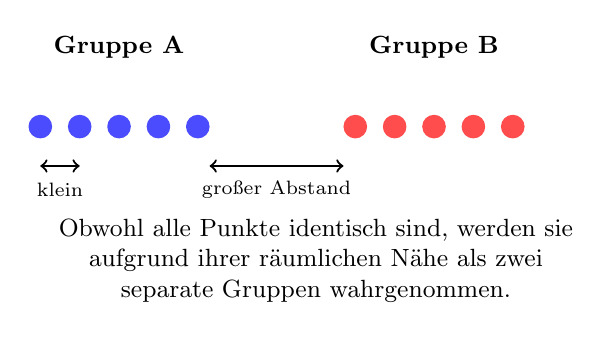
\begin{tikzpicture}[scale=1.0]
    % Left group - perceived as one unit
    \begin{scope}
        \node[font=\small\bfseries] at (1.5, 3) {Gruppe A};
        \fill[blue!70] (0.5, 2) circle (0.15);
        \fill[blue!70] (1.0, 2) circle (0.15);
        \fill[blue!70] (1.5, 2) circle (0.15);
        \fill[blue!70] (2.0, 2) circle (0.15);
        \fill[blue!70] (2.5, 2) circle (0.15);
    \end{scope}
    
    % Right group - perceived as separate unit
    \begin{scope}[xshift=4cm]
        \node[font=\small\bfseries] at (1.5, 3) {Gruppe B};
        \fill[red!70] (0.5, 2) circle (0.15);
        \fill[red!70] (1.0, 2) circle (0.15);
        \fill[red!70] (1.5, 2) circle (0.15);
        \fill[red!70] (2.0, 2) circle (0.15);
        \fill[red!70] (2.5, 2) circle (0.15);
    \end{scope}
    
    % Explanation
    \node[font=\small, align=center] at (4, 0.3){
        Obwohl alle Punkte identisch sind, werden sie\\
        aufgrund ihrer räumlichen Nähe als zwei\\
        separate Gruppen wahrgenommen.
    };
    
    % Distance indicators
    \draw[<->, thick] (2.65, 1.5) -- (4.35, 1.5);
    \node[font=\scriptsize] at (3.5, 1.2) {großer Abstand};
    
    \draw[<->, thick] (0.5, 1.5) -- (1.0, 1.5);
    \node[font=\scriptsize] at (0.75, 1.2) {klein};
    
\end{tikzpicture}
\caption{Illustration des Gestaltprinzips der räumlichen Nähe}
\label{fig:gestalt_proximity}
\end{figure}

Dieses psychologische Prinzip wird in der Dokumentenanalyse algorithmisch umgesetzt: Für jedes erkannte Symbol wird der räumlich \textit{nächstgelegene} Text als zugehörig betrachtet. Die Anwendung von Proximity Heuristiken zur automatischen Layoutanalyse ist ein etabliertes Verfahren in der Dokumentenverarbeitung \cite{Kise1998, Mao2003}.

\subsection{Analogie zur Stücklistenzuordnung}

Für Ingenieure des Maschinenbaus ist das Konzept aus der Arbeit mit technischen Zeichnungen vertraut. Bei einer Explosionsdarstellung mit Positionsnummern ist die Zuordnung zwischen Bauteil und Nummer intuitiv klar: Die Nummer gehört zu dem Bauteil, auf das der Hinweispfeil zeigt oder das sich in räumlicher Nähe befindet (vgl. Abbildung~\ref{fig:parts_list_analogy}). Dieselbe Logik liegt der automatischen Symbol-Text-Verknüpfung zugrunde.

\begin{figure}[H]
\centering
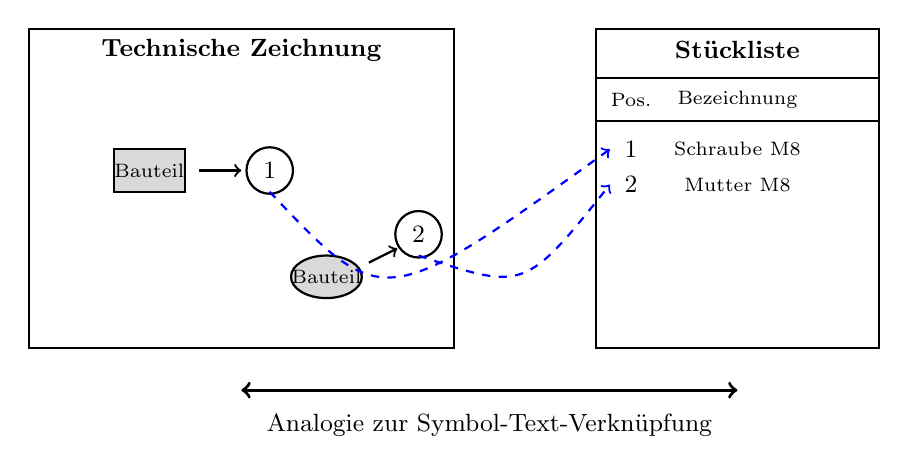
\begin{tikzpicture}[scale=0.9]
    % Technical drawing frame
    \draw[thick] (0,0) rectangle (6,4.5);
    \node[font=\small\bfseries] at (3, 4.2) {Technische Zeichnung};
    
    % Component 1 (schematic bolt)
    \draw[thick, fill=gray!30] (1.2, 2.2) rectangle (2.2, 2.8);
    % KORREKTUR: \scriptsize statt \tiny
    \node[font=\scriptsize] at (1.7, 2.5) {Bauteil};
    \draw[->, thick] (2.4, 2.5) -- (3.0, 2.5);
    \node[circle, draw, thick, fill=white, font=\small] at (3.4, 2.5) {1};
    
    % Component 2 (schematic nut)
    \draw[thick, fill=gray!30] (4.2, 1.0) ellipse (0.5 and 0.3);
    % KORREKTUR: \scriptsize statt \tiny
    \node[font=\scriptsize] at (4.2, 1.0) {Bauteil};
    \draw[->, thick] (4.8, 1.2) -- (5.2, 1.4);
    \node[circle, draw, thick, fill=white, font=\small] at (5.5, 1.6) {2};
    
    % Parts list frame
    \draw[thick] (8, 0) rectangle (12, 4.5);
    \node[font=\small\bfseries] at (10, 4.2) {Stückliste};
    \draw[thick] (8, 3.8) -- (12, 3.8);
    \node[font=\scriptsize] at (8.5, 3.5) {Pos.};
    \node[font=\scriptsize] at (10, 3.5) {Bezeichnung};
    \draw[thick] (8, 3.2) -- (12, 3.2);
    % KORREKTUR: \small statt \scriptsize für die Zahlen
    \node[font=\small] at (8.5, 2.8) {1};
    \node[font=\scriptsize] at (10, 2.8) {Schraube M8};
    % KORREKTUR: \small statt \scriptsize für die Zahlen
    \node[font=\small] at (8.5, 2.3) {2};
    \node[font=\scriptsize] at (10, 2.3) {Mutter M8};
    
    % Connection arrows (dashed)
    \draw[->, dashed, blue, thick] (3.4, 2.2) .. controls (5, 0.5) .. (8.2, 2.8);
    \draw[->, dashed, blue, thick] (5.5, 1.3) .. controls (7, 0.8) .. (8.2, 2.3);
    
    % Analogy label
    \draw[<->, very thick, black] (3, -0.6) -- (10, -0.6);
    \node[font=\small, black] at (6.5, -1.1) {Analogie zur Symbol-Text-Verknüpfung};
    
\end{tikzpicture}
\caption{Zuordnung von Positionsnummern zu Bauteilen in einer Explosionsdarstellung}
\label{fig:parts_list_analogy}
\end{figure}

\subsection{Herausforderung: Rotierte Elemente}

In vielen technischen Zeichnungen folgen Symbole der Geometrie des dargestellten Objekts und können daher in \textbf{beliebigen Winkeln} orientiert sein. Dies stellt eine besondere Herausforderung dar: Die Begriffe \enquote{oberhalb}, \enquote{unterhalb} oder \enquote{rechts von} verlieren bei rotierten Elementen ihre eindeutige Bedeutung im globalen Koordinatensystem. Abbildung~\ref{fig:rotation_problem} illustriert diese Herausforderung: Bei einem horizontal ausgerichteten Symbol ist eindeutig definiert, was \enquote{unterhalb} bedeutet. Bei einem um 45° gedrehten Symbol verliert dieser Begriff jedoch seine eindeutige Bedeutung im globalen Koordinatensystem.

\begin{figure}[H]
\centering
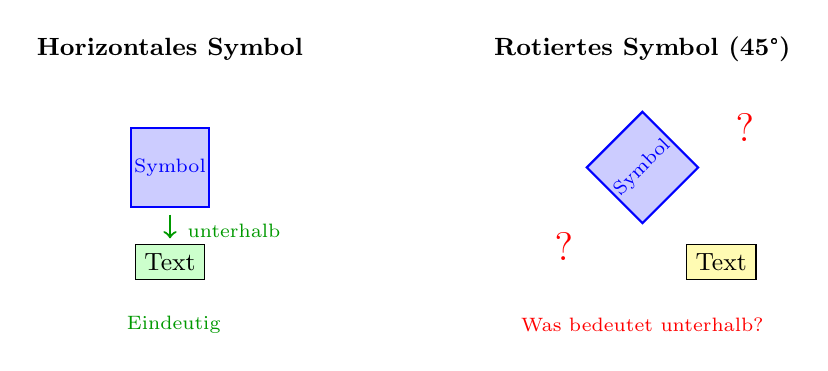
\begin{tikzpicture}[scale=1.0]
    % Left: Horizontal symbol - clear
    \begin{scope}
        \node[font=\small\bfseries] at (1.5, 3.5) {Horizontales Symbol};
        
        % Symbol (horizontal)
        \draw[thick, blue, fill=blue!20] (1, 1.5) rectangle (2, 2.5);
        \node[blue, font=\scriptsize] at (1.5, 2) {Symbol};
        
        % Text below
        \node[rectangle, draw, fill=green!20, font=\small] at (1.5, 0.8) {Text};
        
        % Direction indicator
        \draw[->, thick, green!60!black] (1.5, 1.4) -- (1.5, 1.1);
        \node[font=\scriptsize, green!60!black, right] at (1.6, 1.2) {\enquote{unterhalb}};
        
        \node[font=\scriptsize, green!60!black] at (1.5, 0) {$\checkmark$ Eindeutig};
    \end{scope}
    
    % Right: Rotated symbol - ambiguous
    \begin{scope}[xshift=6cm]
        \node[font=\small\bfseries] at (1.5, 3.5) {Rotiertes Symbol (45°)};
        
        % Symbol (rotated 45 degrees)
        \begin{scope}[rotate around={45:(1.5, 2)}]
            \draw[thick, blue, fill=blue!20] (1, 1.5) rectangle (2, 2.5);
            \node[blue, font=\scriptsize, rotate=45] at (1.5, 2) {Symbol};
        \end{scope}
        
        % Text - where is "below" now?
        \node[rectangle, draw, fill=yellow!30, font=\small] at (2.5, 0.8) {Text};
        
        % Question marks
        \node[font=\Large, red] at (0.5, 1) {?};
        \node[font=\Large, red] at (2.8, 2.5) {?};
        
        \node[font=\scriptsize, red] at (1.5, 0) {Was bedeutet \enquote{unterhalb}?};
    \end{scope}
    
\end{tikzpicture}
\caption{Ambiguität von Richtungsbegriffen bei rotierten Symbolen}
\label{fig:rotation_problem}
\end{figure}

\subsection{Lösung: Lokale Koordinatensysteme}

Die Lösung besteht darin, für jedes Symbol ein eigenes \textbf{lokales Koordinatensystem} zu definieren, das mit der Orientierung des Symbols mitrotiert. In diesem lokalen System haben Richtungsbegriffe wieder eine eindeutige Bedeutung.

Dieses Konzept ist Ingenieuren aus verschiedenen Bereichen vertraut:

\begin{itemize}
    \item \textbf{Technische Mechanik}: Bei der Berechnung von Kräften an einem schräg liegenden Balken transformiert man die Koordinaten in ein lokales System, das mit dem Balken ausgerichtet ist (Hauptachsentransformation) \cite{Gross2021}.
    \item \textbf{CAD-Systeme}: Beim Platzieren von Features auf geneigten Flächen wird automatisch ein lokales Koordinatensystem (User Coordinate System, UCS) verwendet \cite{Zeid2005}.
    \item \textbf{Robotik}: Werkzeugkoordinatensysteme (Tool Center Point, TCP) rotieren mit dem Endeffektor \cite{Siciliano2009}. 
\end{itemize}

\begin{figure}[H]
\centering
\begin{tikzpicture}[
    scale=1.1, 
    >=stealth, 
    font=\small\sffamily,
    % Stile definieren für Konsistenz
    axis/.style={->, thick, black},
    dashed_line/.style={dashed, thin, gray},
    symbol/.style={thick, draw=blue!80!black, fill=blue!5, minimum size=1cm},
    textbox/.style={rectangle, draw=black!60, fill=white, font=\scriptsize, inner sep=3pt}
]

    % --- DEFINITION DER MITTELPUNKTE ---
    % Wir definieren eine feste Höhe (y=1.5) für beide Symbole, damit sie horizontal fluchten
    \coordinate (GlobalCenter) at (1.5, 1.5);
    \coordinate (LocalCenter) at (8.5, 1.5); 

    % ==========================================
    % 1. GLOBALES SYSTEM (Links)
    % ==========================================
    \node[font=\bfseries] at (1.5, 4.2) {Globales System};
    
    % Globale Achsen (stehen fest im Raum)
    \draw[axis] (-0.5, 0) -- (3.5, 0) node[right] {$x_{\text{global}}$};
    \draw[axis] (0, -0.5) -- (0, 3.5) node[above] {$y_{\text{global}}$};
    
    % Das Symbol (gedreht um seinen Mittelpunkt)
    \begin{scope}[rotate around={30:(GlobalCenter)}]
        % Das Symbol selbst
        \node[symbol, transform shape] (sym1) at (GlobalCenter) {Symbol};
        
        % Die "gedachte" lokale Achse (gestrichelt), auf der der Text eigentlich liegen soll
        \draw[dashed, blue!50] (GlobalCenter) -- ++(0, 2.2);
        
        % Der Text (rotiert mit)
        \node[textbox, transform shape] (txt1) at ($(GlobalCenter)+(0, 1.8)$) {Text};
    \end{scope}

    % Das PROBLEM visualisieren:
    % Wir zeichnen die globalen x/y Abstände ein um zu zeigen, dass es kompliziert ist
    \draw[dashed_line, red] (GlobalCenter) -- (1.5, 3.05) -- (0.7, 3.05);
    \node[text=red, font=\scriptsize, align=left] at (2.8, 2.5) {Komplizierte\\Koordinaten?\\$(\Delta x, \Delta y)$};
    \draw[->, red, bend right=20] (2.0, 2.5) to (txt1.east);


    % ==========================================
    % PFEIL: TRANSFORMATION (Mitte)
    % ==========================================
    \draw[->, very thick, black!70] (4.0, 1.5) -- (6.0, 1.5);
    \node[align=center, font=\footnotesize, above] at (5.0, 1.6) {Koordinaten-\\transformation};


    % ==========================================
    % 2. LOKALES SYSTEM (Rechts)
    % ==========================================
    \node[font=\bfseries] at (8.5, 4.2) {Lokales System};
    
    % Lokale Achsen (gehen DURCH das Symbol)
    \draw[axis] (LocalCenter) -- ++(2.0, 0) node[right] {$x_{\text{lokal}}$};
    \draw[axis] (LocalCenter) -- ++(0, 2.0) node[above] {$y_{\text{lokal}}$};
    % Die negativen Achsen etwas kürzer andeuten
    \draw[thick, black] (LocalCenter) -- ++(-1.0, 0);
    \draw[thick, black] (LocalCenter) -- ++(0, -1.0);
    
    % Das Symbol (Gerade, im Ursprung des lokalen Systems)
    \node[symbol] (sym2) at (LocalCenter) {Symbol};
    
    % Der Text (Gerade, exakt auf der y-Achse)
    \node[textbox] (txt2) at ($(LocalCenter)+(0, 1.8)$) {Text};
    
    % Die LÖSUNG visualisieren:
    % Ein grüner Maßpfeil direkt auf der Achse
    \draw[<->, green!60!black, thick] ($(sym2.north)+(0.1,0)$) -- ($(txt2.south)+(0.1,0)$);
    \node[text=green!60!black, font=\scriptsize, right] at (8.7, 2.5) {Einfacher Abstand};
    \node[text=green!60!black, font=\scriptsize, right] at (8.7, 2.1) {$(0, \Delta y)$};

\end{tikzpicture}
\caption{Transformation vom globalen ins lokale Koordinatensystem eines Symbols}
\label{fig:local_coordinates_clear}
\end{figure}


Wie in Abbildung~\ref{fig:local_coordinates_clear} dargestellt, werden durch die Transformation ins lokale System Richtungsbeziehungen wieder eindeutig: Der Begriff \enquote{oberhalb} bezieht sich nun auf die positive $y_{\text{lokal}}$-Achse, unabhängig von der globalen Orientierung des Symbols.
Die mathematische Umsetzung dieser Transformation, eine Rotation des Koordinatensystems um den Winkel des Symbols, wird in Kapitel~\ref{chap:implementierung}, Abschnitt \ref{sec:Koordinatentransformation} detailliert beschrieben.

\subsection{Klassenspezifische Suchstrategien}

In der Praxis variieren die räumlichen Beziehungen zwischen Symbol und Text je nach Objekttyp. Dies spiegelt die Zeichnungskonventionen wider, die sich in verschiedenen Domänen etabliert haben:

\begin{table}[H]
\centering
\renewcommand{\arraystretch}{1.3}
\begin{tabular}{|p{3cm}|p{4cm}|p{6cm}|}
\hline
\textbf{Objekttyp} & \textbf{Typische Textposition} & \textbf{Begründung} \\
\hline
Signal & Unterhalb des Symbols & Signalbezeichnungen stören nicht die Gleisdarstellung \\
\hline
Kilometerstein & Direkt am Markierungspunkt & Kompakte Darstellung der Streckenposition \\
\hline
Weiche & Variable Positionen & Komplexe Geometrie erfordert flexible Platzierung \\
\hline
\end{tabular}
\caption{Domänenspezifische Konventionen für Textpositionen relativ zu Symbolen}
\label{tab:text_position_conventions}
\end{table}

Diese Konventionen werden als \textbf{Domänenwissen} in das System integriert und ermöglichen eine gezieltere Suche nach zusammengehörigen Elementen. Derartige domänenspezifische Layoutregeln sind charakteristisch für technische Dokumentationen und folgen etablierten Zeichnungsnormen \cite{DIN_ISO_128, Hoischen2022}. 


%==============================================================================
\section{Änderungserkennung zwischen Dokumentversionen}
\label{sec:change_detection}

Technische Dokumente unterliegen einem kontinuierlichen Änderungsprozess. Im Verlauf eines Projekts werden Pläne mehrfach überarbeitet: Elemente werden hinzugefügt, verschoben oder entfernt; Bezeichnungen werden korrigiert. Die systematische Erfassung dieser Änderungen ist essenziell für die Qualitätssicherung und Nachvollziehbarkeit im Engineering-Prozess.

\subsection{Motivation: Das Revisionswesen}

In der industriellen Praxis folgt die Dokumentenlenkung definierten Prozessen gemäß Qualitätsmanagementsystemen wie DIN EN ISO 9001 \cite{DINISO9001}. Jede Änderung an einer technischen Zeichnung muss:

\begin{itemize}
    \item \textbf{Dokumentiert} werden (Was wurde geändert?)
    \item \textbf{Begründet} werden (Warum wurde geändert?)
    \item \textbf{Freigegeben} werden (Wer hat die Änderung geprüft?)
\end{itemize}

Die manuelle Identifikation von Änderungen zwischen zwei Planversionen, das sogenannte \enquote{Rödeln} ist zeitaufwändig und fehleranfällig, insbesondere bei umfangreichen Dokumenten mit hunderten von Elementen.

\subsection{Analogie: Stücklistenvergleich}

Das Konzept der Änderungserkennung ist Ingenieuren aus dem Stücklistenwesen bekannt. Wenn sich eine Baugruppe ändert, muss die zugehörige Stückliste (Bill of Materials, BOM) aktualisiert werden \cite{stark2022}. Ein BOM-Vergleich identifiziert:

\begin{itemize}
    \item \textbf{Neue Positionen}: Bauteile, die hinzugekommen sind
    \item \textbf{Entfallene Positionen}: Bauteile, die entfernt wurden
    \item \textbf{Geänderte Positionen}: Bauteile mit modifizierten Attributen (Menge, Material, etc.)
\end{itemize}

Dieselbe Logik lässt sich auf technische Zeichnungen übertragen.

\subsection{Kategorisierung von Änderungen}

Abbildung~\ref{fig:revision_example} zeigt typische Änderungen zwischen zwei Dokumentversionen: Symbol S3 wurde hinzugefügt, Symbol S2 wurde entfernt, und Symbol W1 wurde an eine neue Position verschoben.

\begin{figure}[H]
\centering
\begin{tikzpicture}[
    scale=0.95, 
    font=\small\sffamily, % Serifenlose Schrift für technische Diagramme
    >=stealth,            % Professionelle Pfeilspitzen
    % --- STILE ---
    % Container: Schwarz, weißer Hintergrund (oder transparent), keine runden Ecken für technischen Look
    container/.style={draw=black, thick, fill=white, minimum width=4.5cm, minimum height=5.5cm, align=center},
    % Objekte
    symbol_circle/.style={circle, draw=black, thick, minimum size=0.8cm, inner sep=0pt},
    symbol_rect/.style={rectangle, draw=black, thick, minimum width=1.4cm, minimum height=0.7cm},
    % Status-Texte
    status_text/.style={font=\scriptsize\bfseries}
]

    % ==========================================
    % VERSION A (ALT)
    % ==========================================
    \node[container] (boxA) at (0,0) {};
    \node[below=2pt] at (boxA.north) {\textbf{Version A} (Alt)};

    % S1 (Bleibt gleich)
    \node[symbol_circle, fill=blue!10] (s1_a) at ($(boxA.center)+(-1, 1.5)$) {S1};
    
    % S2 (Wird entfernt)
    \node[symbol_circle, fill=blue!10] (s2_a) at ($(boxA.center)+(0.8, 0.5)$) {S2};
    % Durchstreichen (Klassisches technisches "X")
    \draw[red!70!black, thick] (s2_a.north west) -- (s2_a.south east);
    \draw[red!70!black, thick] (s2_a.north east) -- (s2_a.south west);
    \node[status_text, text=red!70!black, below=0.1cm of s2_a] {ENTFERNT};

    % W1 (Ursprungsposition) - Gestrichelt ("Ghost")
    \node[symbol_rect, draw=black!60, dashed, fill=none] (w1_a) at ($(boxA.center)+(-0.5, -1.5)$) {\textcolor{gray}{W1}};


    % ==========================================
    % PFEIL: REVISION (Mitte)
    % ==========================================
    % Schlichter, schwarzer Pfeil
    \draw[->, thick, black] ($(boxA.east)+(0.2,0)$) -- ($(boxA.east)+(2.8,0)$) 
        node[midway, above] {Revision};


    % ==========================================
    % VERSION B (NEU)
    % ==========================================
    \node[container, right=3cm of boxA] (boxB) {};
    \node[below=2pt] at (boxB.north) {\textbf{Version B} (Neu)};

    % S1 (Unverändert)
    \node[symbol_circle, fill=blue!10] (s1_b) at ($(boxB.center)+(-1, 1.5)$) {S1};

    % S3 (NEU)
    \node[symbol_circle, draw=black, fill=green!10] (s3_b) at ($(boxB.center)+(0.8, 0.8)$) {S3};
    % Label "NEU"
    \node[status_text, text=green!40!black, right=0.3cm of s3_b] (neu_label) {NEU};
    \draw[->, green!40!black, thin] (neu_label.west) -- (s3_b.east);

    % W1 (Neue Position) - Voll gezeichnet
    \node[symbol_rect, fill=red!10] (w1_b) at ($(boxB.center)+(0.8, -1.5)$) {W1};


    % ==========================================
    % VERSCHIEBUNG (Pfeil)
    % ==========================================
    % Schwarzer, gepunkteter Pfeil von der alten zur neuen Position
    \draw[->, dotted, thick, black, bend right=25] 
        (w1_a.east) to node[midway, above, sloped, font=\scriptsize, text=black, fill=white, inner sep=1pt] {VERSCHOBEN} (w1_b.west);

\end{tikzpicture}
\caption{Schematische Darstellung von Änderungen zwischen zwei Planversionen.}
\label{fig:revision_example}
\end{figure}

\begin{table}[H]
\centering
\renewcommand{\arraystretch}{1.4}
\begin{tabular}{|p{2.5cm}|p{5cm}|p{5.5cm}|}
\hline
\textbf{Änderungstyp} & \textbf{Definition} & \textbf{Praktisches Beispiel} \\
\hline
\textbf{Hinzufügung} & Element existiert nur in der neuen Version & Ein zusätzliches Signal wurde installiert \\
\hline
\textbf{Entfernung} & Element existiert nur in der alten Version & Ein Haltepunkt wurde stillgelegt \\
\hline
\textbf{Modifikation} & Element existiert in beiden Versionen, aber mit geänderten Attributen & Die Bezeichnung eines Signals wurde korrigiert \\
\hline
\textbf{Verschiebung} & Element existiert in beiden Versionen, aber an unterschiedlicher Position & Ein Symbol wurde im Plan neu platziert \\
\hline
\end{tabular}
\caption{Die vier Grundtypen von Änderungen zwischen Dokumentversionen}
\label{tab:change_categories}
\end{table}

\subsection{Prinzip: Identifikation durch eindeutige Merkmale}

Um Änderungen automatisch zu erkennen, muss zunächst festgestellt werden, welche Elemente in beiden Versionen \enquote{dasselbe} Objekt darstellen. Dies erfolgt über \textbf{eindeutige Identifikationsmerkmale} -- vergleichbar mit Artikelnummern in einer Stückliste oder Sachnummern in einem PDM-System \cite{stark2022}.

Für technische Zeichnungen können solche Identifikatoren aus den Objektattributen abgeleitet werden. Ein Signal mit der Bezeichnung \enquote{AS102} erhält beispielsweise eine eindeutige Kennung, die aus Objekttyp und Bezeichnung zusammengesetzt wird.

\subsection{Mengentheoretische Betrachtung}

Mit eindeutigen Identifikatoren lässt sich die Änderungserkennung konzeptionell auf Mengenoperationen zurückführen:

\begin{figure}[H]
\centering
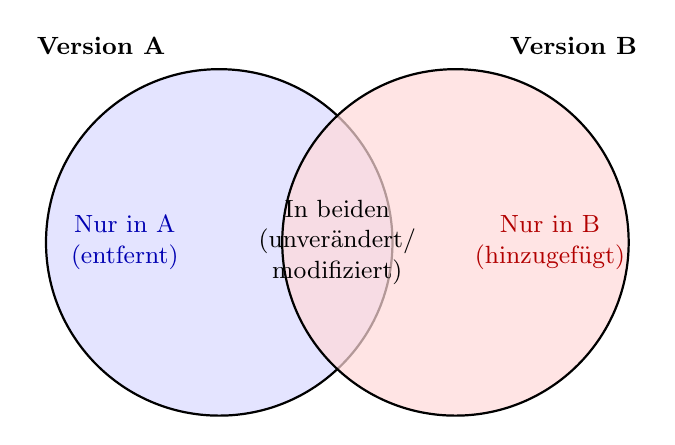
\begin{tikzpicture}[scale=1.0]
    % Venn diagram
    \draw[thick, fill=blue!15, fill opacity=0.7] (0, 0) circle (2.2);
    \draw[thick, fill=red!15, fill opacity=0.7] (3, 0) circle (2.2);
    
    % Labels
    \node[font=\small\bfseries] at (-1.5, 2.5) {Version A};
    \node[font=\small\bfseries] at (4.5, 2.5) {Version B};
    
    % Set regions with descriptions
    \node[font=\small, blue!70!black, align=center] at (-1.2, 0) {Nur in A\\(entfernt)};
    
    \node[font=\small, align=center] at (1.5, 0) {In beiden\\(unverändert/\\modifiziert)};
    
    \node[font=\small, red!70!black, align=center] at (4.2, 0) {Nur in B\\(hinzugefügt)};
    
\end{tikzpicture}
\caption{Änderungserkennung als Mengenvergleich zweier Dokumentversionen}
\label{fig:set_comparison_concept}
\end{figure}

Für Elemente in der Schnittmenge (gleiche Kennung in beiden Versionen) muss zusätzlich geprüft werden, ob sich ihre Attribute geändert haben. Die algorithmische Umsetzung dieser Konzepte wird in Kapitel~\ref{chap:implementierung}, Abschnitt \ref{subsec:vergleichundänderung} beschrieben.


%==============================================================================
\section{Konfigurationsbasierte Systemanpassung}
\label{sec:config_based_adaptation}

Ein wesentliches Qualitätsmerkmal technischer Software ist ihre \textbf{Anpassbarkeit} an unterschiedliche Einsatzszenarien. In der industriellen Praxis variieren Symbolvarianten, Bezeichnungskonventionen und Validierungsregeln zwischen verschiedenen Kunden, Projekten oder Regionen. Eine starre, im Programmcode verankerte Logik würde für jede Anpassung eine Softwareänderung erfordern.

\subsection{Das Problem der Domänenspezifität}

Technische Zeichnungen folgen zwar grundlegenden Normen (z.\,B. DIN für Zeichnungselemente), weisen aber in der Praxis erhebliche Variabilität auf:

\begin{itemize}
    \item \textbf{Kundenspezifische Symbole}: Verschiedene Unternehmen verwenden unterschiedliche Darstellungen für dieselbe technische Funktion
    \item \textbf{Regionale Konventionen}: Bezeichnungsschemata variieren zwischen Ländern
    \item \textbf{Historische Entwicklung}: Ältere Dokumente folgen anderen Standards als aktuelle
\end{itemize}

Abbildung~\ref{fig:domain_variability} verdeutlicht das Problem: Drei verschiedene Kunden verwenden unterschiedliche Symboldarstellungen und Bezeichnungsformate für dieselbe technische Funktion. Ein starres System müsste für jede Variante angepasst werden.
\begin{figure}[H]
\centering
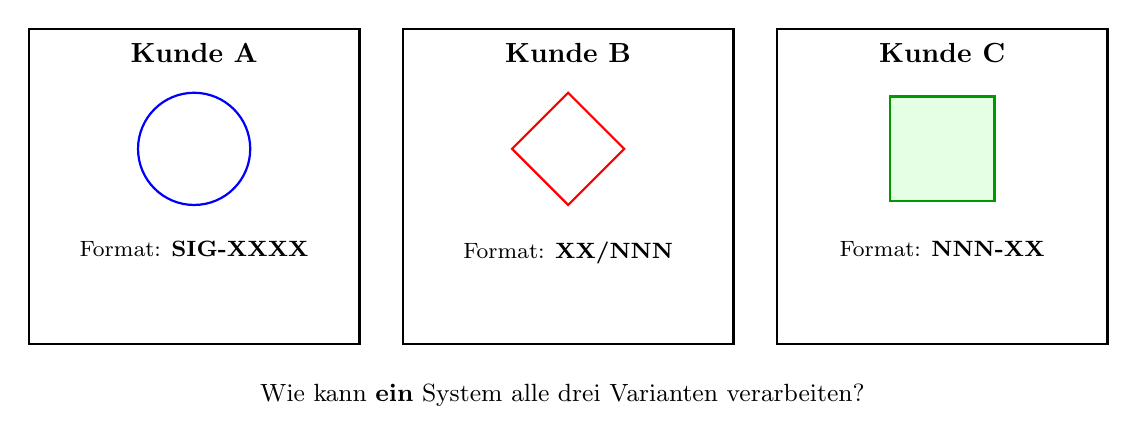
\begin{tikzpicture}[
    scale=0.95,
    font=\small\sffamily,
    % Stile für Konsistenz
    container/.style={draw=black, thick, fill=white, minimum width=4.2cm, minimum height=4cm},
    title/.style={font=\bfseries, below=2pt},
    fmt_text/.style={font=\footnotesize, align=center, anchor=north, yshift=-0.2cm}
]

    % ==========================================
    % KUNDE A (Kreis)
    % ==========================================
    \begin{scope}
        \node[container] (boxA) at (0,0) {};
        \node[title] at (boxA.north) {Kunde A};
        
        % Symbol vergrößert (Radius 0.5 -> 0.75)
        \draw[thick, blue] (0, 0.5) circle (0.75);
        
        % Text vergrößert und positioniert
        \node[fmt_text] at (0, -0.4) {Format: \textbf{SIG-XXXX}};
    \end{scope}
    
    % ==========================================
    % KUNDE B (Raute)
    % ==========================================
    \begin{scope}[xshift=5cm]
        \node[container] (boxB) at (0,0) {};
        \node[title] at (boxB.north) {Kunde B};
        
        % Symbol vergrößert (Skaliert um Faktor ~1.5)
        \draw[thick, red] (0, 1.25) -- (0.75, 0.5) -- (0, -0.25) -- (-0.75, 0.5) -- cycle;
        
        \node[fmt_text] at (0, -0.4) {Format: \textbf{XX/NNN}};
    \end{scope}
    
    % ==========================================
    % KUNDE C (Quadrat)
    % ==========================================
    \begin{scope}[xshift=10cm]
        \node[container] (boxC) at (0,0) {};
        \node[title] at (boxC.north) {Kunde C};
        
        % Symbol vergrößert (1x1cm -> 1.4x1.4cm)
        \draw[thick, green!60!black, fill=green!10] (-0.7, -0.2) rectangle (0.7, 1.2);
        
        \node[fmt_text] at (0, -0.4) {Format: \textbf{NNN-XX}};
    \end{scope}
    
    % ==========================================
    % PROBLEMSTELLUNG
    % ==========================================
    \node[font=\small, align=center] at (5, -2.8) {
        Wie kann \textbf{ein} System alle drei Varianten verarbeiten?
    };
    
\end{tikzpicture}
\caption{Variabilität von Symboldarstellungen und Bezeichnungskonventionen.}
\label{fig:domain_variability}
\end{figure}

\subsection{Lösung: Trennung von Code und Konfiguration}

Die Lösung besteht in der strikten Trennung zwischen:

\begin{enumerate}
    \item \textbf{Programmlogik} (Code): Die allgemeinen Algorithmen für Erkennung, Verknüpfung und Validierung, die bleiben für alle Anwendungsfälle gleich
    
    \item \textbf{Domänenwissen} (Konfiguration): Die spezifischen Regeln, Parameter und Erwartungswerte, die werden in einem zentralen Konfigurationsmodul definiert
\end{enumerate}

Dieses Prinzip der \textit{Separation of Concerns} ist ein fundamentales Konzept der Softwarearchitektur \cite{Dijkstra1982} und ermöglicht die Anpassung des Systems durch Änderung weniger, klar strukturierter Parameter.

Dieses Prinzip ist Ingenieuren aus verschiedenen Bereichen bekannt:

\begin{itemize}
    \item \textbf{Parametrische CAD-Modelle}: Die Geometrie wird durch Parameter gesteuert, nicht durch hartcodierte Maße \cite{Shah1995}
    \item \textbf{SPS-Programmierung}: Prozessparameter werden in Datenbausteinen (DBs) abgelegt, nicht im Programmcode \cite{IEC61131}
    \item \textbf{FEM-Software}: Materialparameter werden in Bibliotheken gepflegt, nicht im Solver \cite{Zienkiewicz2013}
\end{itemize}

\begin{figure}[H]
\centering
\begin{tikzpicture}[
    scale=0.95,
    font=\sffamily,
    % Styles für Konsistenz
    box/.style={thick, rectangle, minimum height=4.5cm, minimum width=5.5cm, align=center},
    title/.style={font=\bfseries\small, anchor=north, yshift=-0.2cm},
    content/.style={font=\small, align=left, anchor=center, text width=4.8cm} % text width sorgt für sauberen Umbruch/Ausrichtung
]

    % ==========================================
    % Programmcode (Fest) - Links
    % ==========================================
    \node[box, fill=blue!10, draw=blue!50!black] (code) at (0, 0) {};
    
    % Titel
    \node[title, text=blue!50!black] at (code.north) {Programmcode (fest)};
    
    % Inhalt (Liste) - Größerer Text (\small) und mehr Abstand
    \node[content] at (code.center) {
        $\bullet$ Erkennungsalgorithmus\\[0.1cm]
        $\bullet$ Verknüpfungslogik\\[0.1cm]
        $\bullet$ Validierungsframework\\[0.1cm]
        $\bullet$ Exportfunktionen
    };
    
    
    % ==========================================
    % Verbindungspfeil (Mitte)
    % ==========================================
    % Wir definieren den rechten Knoten relativ zum linken, für flexible Positionierung
    \node[box, fill=green!10, draw=green!40!black, right=2cm of code] (config) {};
    
    \draw[->, very thick, black] (code.east) -- (config.west) 
        node[midway, above, font=\small] {liest};
    
    
    % ==========================================
    % Konfiguration (Anpassbar) - Rechts
    % ==========================================
    % Titel
    \node[title, text=green!40!black] at (config.north) {Konfiguration (anpassbar)};
    
    % Inhalt
    \node[content] at (config.center) {
        $\bullet$ Symbolklassen \& Namen\\[0.1cm]
        $\bullet$ Erwartete Textformate\\[0.1cm]
        $\bullet$ Suchradien\\[0.1cm]
        $\bullet$ Validierungsregeln
    };
    
\end{tikzpicture}
\caption{Architekturprinzip der Trennung von Programmlogik und Konfiguration.}
\label{fig:code_config_separation}
\end{figure}


Wie in Abbildung~\ref{fig:code_config_separation} dargestellt, liest der unveränderliche Programmcode die domänenspezifischen Parameter aus einem externen Konfigurationsmodul. Anpassungen an neue Kundenanforderungen erfordern dadurch keine Codeänderungen.
\subsection{Typische Konfigurationsparameter}

Für ein Dokumentenanalysesystem sind folgende Parameter typischerweise konfigurierbar:

\begin{table}[H]
\centering
\renewcommand{\arraystretch}{1.3}
\begin{tabular}{|p{3.5cm}|p{4.5cm}|p{5cm}|}
\hline
\textbf{Kategorie} & \textbf{Beispiel} & \textbf{Zweck} \\
\hline
Konfidenzschwellen & Klassenspezifische Mindestkonfidenzen & Präzisions-/Recall-Balance je Klasse \\
\hline
Verknüpfungsregeln & Suchrichtung, Distanzmultiplikatoren & Steuerung der Symbol-Text-Zuordnung \\
\hline
NMS-Parameter & Klassenspezifische IoU-Schwellen & Unterdrückung von Duplikaten \\
\hline
OCR-Vorverarbeitung & Schärfung, Rauschunterdrückung & Optimierung der Texterkennung \\
\hline
\end{tabular}
\caption{Kategorien konfigurierbarer Parameter}
\label{tab:config_parameters}
\end{table}

\subsection{Klassenspezifische Parameter}

Ein wesentliches Merkmal ist die \textbf{klassenspezifische Parametrisierung}: Jede Symbolklasse kann eigene optimierte Werte erhalten, da verschiedene Klassen unterschiedliche Erkennungsschwierigkeiten aufweisen:

\begin{itemize}
    \item Klassen mit hoher Erkennungssicherheit (z.\,B. geometrisch eindeutige Symbole) können niedrigere Konfidenzschwellen verwenden
    \item Klassen mit vielen Falsch-Positiven erfordern strengere Schwellen
    \item Die Suchrichtung für zugehörigen Text variiert je nach typischer Anordnung im Dokument
\end{itemize}

\subsection{Orientierungsabhängige Verarbeitung}

Zusätzlich zur Klassenspezifik werden Parameter nach \textbf{Textorientierung} differenziert. Horizontaler und schräger Text erfordern unterschiedliche OCR-Vorverarbeitung:

\begin{itemize}
    \item \textbf{Kardinale Orientierung} (0°, 90°, 180°, 270°): Standardparameter für achsparallelen Text
    \item \textbf{Anguläre Orientierung} (schräg): Angepasste Parameter mit erhöhter Vorverarbeitung
\end{itemize}

Diese Unterscheidung ermöglicht optimale Erkennungsraten unabhängig von der Textausrichtung im Dokument.

Die konkrete Struktur des Konfigurationsmoduls wird in Kapitel~\ref{chap:konzeption} und seine Verarbeitung in Kapitel~\ref{chap:implementierung} beschrieben.


%==============================================================================
\section{Rückverfolgbarkeit und Qualitätssicherung}
\label{sec:traceability_qa}

Bei der automatisierten Extraktion von Daten, insbesondere in sicherheitsrelevanten Domänen, ist die \textbf{Rückverfolgbarkeit} der Ergebnisse von fundamentaler Bedeutung. Jeder extrahierte Datensatz muss auf seine Quelle zurückführbar sein, um die Korrektheit überprüfen und bei Fehlern die Ursache identifizieren zu können.

\subsection{Definition und Bedeutung}

\textbf{Rückverfolgbarkeit} (\textit{Traceability}) bezeichnet die Fähigkeit, für jedes Ergebnis dessen Herkunft und Entstehungsweg nachzuvollziehen \cite{Gotel1994}. In der Qualitätssicherung ist dieses Prinzip fest verankert -- vergleichbar mit:

\begin{itemize}
    \item \textbf{Chargenrückverfolgung} in der Fertigung (jedes Bauteil ist auf seine Herkunft zurückführbar) \cite{EU178_2002}
    \item \textbf{Audit Trail} in der Prozessindustrie (jede Parameteränderung wird protokolliert) \cite{FDA21CFR11}
    \item \textbf{Requirements Tracing} in der Systementwicklung (jede Anforderung ist bis zur Implementierung nachverfolgbar) \cite{Pohl2010}
\end{itemize}

\subsection{Komponenten der Rückverfolgbarkeit}

Für ein Dokumentenanalysesystem bedeutet Rückverfolgbarkeit, dass zu jedem extrahierten Datensatz folgende Informationen verfügbar sein müssen. Abbildung~\ref{fig:traceability_principle} zeigt das Prinzip: Jeder extrahierte Datensatz enthält neben dem eigentlichen Inhalt auch Metadaten zur Quelldatei, Position und Erkennungskonfidenz, die eine Rückverfolgung zur Originalstelle im Dokument ermöglichen.
\begin{figure}[H]
\centering
\begin{tikzpicture}[
    scale=0.95,
    font=\sffamily,
    >=stealth,
    % Stile definieren
    doc_frame/.style={draw=black, thick, fill=white, minimum width=4.5cm, minimum height=5.5cm},
    data_frame/.style={draw=black, thick, fill=blue!5, minimum width=6.5cm, minimum height=5cm, rounded corners=2pt},
    highlight_box/.style={draw=red!80!black, thick, fill=red!10, minimum width=2.8cm, minimum height=1.2cm, align=center, font=\footnotesize},
    arrow_label/.style={font=\small, align=center}
]

    % ==========================================
    % 1. QUELLDOKUMENT (Links)
    % ==========================================
    \node[doc_frame] (source) at (0,0) {};
    \node[below=2pt, font=\bfseries] at (source.north) {Quelldokument};
    
    % Roter Kasten (Vergrößert)
    \node[highlight_box] (element) at (0, 0.5) {erkanntes\\Element};
    
    
    % ==========================================
    % PFEIL: EXTRAKTION (Mitte)
    % ==========================================
    \draw[->, very thick, black!80] (source.east) -- ($(source.east)+(2.5,0)$) 
        node[midway, above, font=\small] {Extraktion};


    % ==========================================
    % 2. EXTRAHIERTER DATENSATZ (Rechts)
    % ==========================================
    \node[data_frame, right=2.5cm of source] (dataset) {};
    \node[below=2pt, font=\bfseries] at (dataset.north) {Extrahierter Datensatz};
    
    % Inhalt (Schriftart \small und mehr Zeilenabstand)
    \node[font=\small, align=left, anchor=center] at (dataset.center) {
        \textbf{Inhalt}: AS102\\[0.3em]
        \textbf{Klasse}: Signal\\[0.3em]
        \textbf{Quelle}: Plan\_v3.pdf, Seite 2\\[0.3em]
        \textbf{Position}: (1024, 768) px\\[0.3em]
        \textbf{Konfidenz}: 94\%
    };
    
    
    % ==========================================
    % RÜCKVERFOLGUNG (Pfeil unten)
    % ==========================================
    % Startet unten am Datensatz und geht zum roten Element
    \draw[->, thick, dashed, green!50!black] 
        ($(dataset.south)+(-1,0)$) 
        .. controls ($(dataset.south)+(-1,-1.5)$) and ($(source.south)+(0,-1.5)$) .. 
        (element.south);
        
    % Label für den Pfeil (Besser lesbar)
    \node[font=\small, text=green!50!black, fill=white, inner sep=2pt] at ($(source.south east)!0.5!(dataset.south west) + (0,-1.1)$) {Rückverfolgung zur Quelle};
    
\end{tikzpicture}
\caption{Struktur eines rückverfolgbaren Datensatzes mit Quellenmetadaten.}
\label{fig:traceability_principle}
\end{figure}

\begin{table}[H]
\centering
\renewcommand{\arraystretch}{1.3}
\begin{tabular}{|p{3.5cm}|p{9.5cm}|}
\hline
\textbf{Information} & \textbf{Beschreibung} \\
\hline
Quellenreferenz & Dateiname, Seitennummer, Dokumentversion \\
\hline
Positionsangabe & Koordinaten des erkannten Elements im Originaldokument \\
\hline
Verarbeitungsmetadaten & Verwendete Algorithmen, Zeitstempel der Verarbeitung \\
\hline
Konfidenzinformation & Sicherheit der Erkennung als quantitativer Wert \\
\hline
\end{tabular}
\caption{Wesentliche Metadaten für die Rückverfolgbarkeit}
\label{tab:traceability_metadata}
\end{table}

\subsection{Qualitätssicherung durch Validierung}

Automatische Erkennungssysteme erreichen nie 100\% Genauigkeit. Fehler können in jeder Stufe der Verarbeitungskette auftreten. Um die Auswirkungen solcher Fehler zu minimieren, ist eine \textbf{mehrstufige Validierung} erforderlich.

Das Grundprinzip besteht darin, jedes Ergebnis mehreren unabhängigen Plausibilitätsprüfungen zu unterziehen \cite{Juran1988}:

\begin{itemize}
    \item \textbf{Formatprüfung}: Entspricht das Ergebnis dem erwarteten syntaktischen Muster?
    \item \textbf{Wertebereichsprüfung}: Liegt der Wert innerhalb plausibler Grenzen?
    \item \textbf{Kontextprüfung}: Ist das Ergebnis im räumlichen/logischen Kontext plausibel?
\end{itemize}

\subsection{Umgang mit unsicheren Ergebnissen}

Moderne Erkennungssysteme liefern zusammen mit dem Ergebnis einen \textbf{Konfidenzwert}, der die Sicherheit der Erkennung quantifiziert \cite{Guo2017}. Diese Information kann genutzt werden, um Ergebnisse zu klassifizieren. Abbildung~\ref{fig:confidence_zones} zeigt eine typische Einteilung: Ergebnisse mit hoher Konfidenz (über 90\%) werden automatisch akzeptiert, mittlere Werte erfordern eine visuelle Kontrolle, und niedrige Werte werden zur manuellen Prüfung markiert.

\begin{figure}[H]
\centering
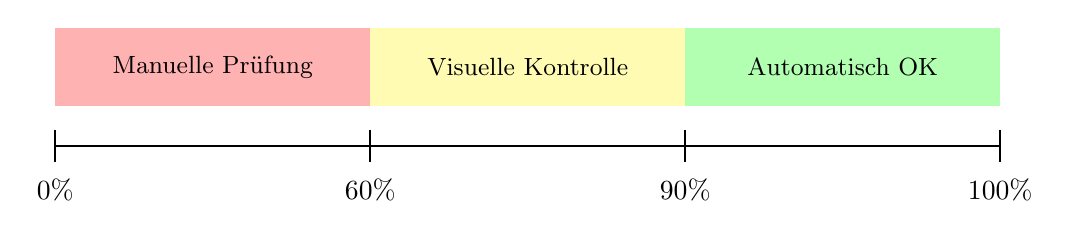
\begin{tikzpicture}[scale=1.0]
    % Confidence scale
    \draw[thick] (0, 0) -- (12, 0);
    
    % Markers
    \draw[thick] (0, -0.2) -- (0, 0.2);
    \draw[thick] (4, -0.2) -- (4, 0.2);
    \draw[thick] (8, -0.2) -- (8, 0.2);
    \draw[thick] (12, -0.2) -- (12, 0.2);
    
    % Labels
    \node[below] at (0, -0.3) {0\%};
    \node[below] at (4, -0.3) {60\%};
    \node[below] at (8, -0.3) {90\%};
    \node[below] at (12, -0.3) {100\%};
    
    % Zones
    \fill[red!30] (0, 0.5) rectangle (4, 1.5);
    \fill[yellow!30] (4, 0.5) rectangle (8, 1.5);
    \fill[green!30] (8, 0.5) rectangle (12, 1.5);
    
    % Zone labels
    \node[font=\small] at (2, 1) {Manuelle Prüfung};
    \node[font=\small] at (6, 1) {Visuelle Kontrolle};
    \node[font=\small] at (10, 1) {Automatisch OK};
    
\end{tikzpicture}
\caption{Konfidenzbasierte Klassifikation von Erkennungsergebnissen}
\label{fig:confidence_zones}
\end{figure}

\subsection{Human-in-the-Loop: Der Mensch als finale Instanz}

Unabhängig von der Leistungsfähigkeit automatischer Systeme bleibt der \textbf{Mensch die finale Prüfinstanz}. Dieses Prinzip, in der Informatik als \enquote{Human-in-the-Loop} bezeichnet \cite{Monarch2021}, ist besonders für sicherheitsrelevante Anwendungen unverzichtbar.

Das System sollte daher:
\begin{itemize}
    \item Unsichere Ergebnisse \textit{markieren}, nicht automatisch verwerfen
    \item Dem Anwender eine \textit{effiziente Überprüfung} ermöglichen (z.\,B. durch Navigation zur Quellposition)
    \item \textit{Korrekturmöglichkeiten} bieten, ohne den Gesamtprozess neu starten zu müssen
\end{itemize}

Die konkrete Implementierung der Validierungslogik und der Benutzerinteraktion wird in Kapitel~\ref{chap:implementierung}, Abschnitte \ref{sec:validierungundsicherung} und \ref{sec:benutzeroberfläche} beschrieben.

\subsection{Zusammenfassung: Theoretische Grundlagen}

Die in diesem Kapitel dargestellten theoretischen Konzepte bilden das Fundament für die praktische Implementierung des Extraktionssystems:

\begin{itemize}
    \item \textbf{Objekterkennung} (Abschnitt \ref{sec:objekterkennung}): Neuronale Netze für die Detektion von Symbolen
    \item \textbf{Texterkennung} (Abschnitt \ref{sec:ocr}): OCR-Verfahren für die Extraktion von Beschriftungen
    \item \textbf{Räumliche Verknüpfung} (Abschnitt \ref{sec:spatial_relations}): Proximale Algorithmen mit lokalen Koordinatensystemen
    \item \textbf{Änderungserkennung} (Abschnitt \ref{sec:change_detection}): Mengenbasierter Vergleich von Dokumentversionen
    \item \textbf{Konfigurierbarkeit} (Abschnitt \ref{sec:config_based_adaptation}): Trennung von Code und Domänenwissen
    \item \textbf{Qualitätssicherung} (Abschnitt \ref{sec:traceability_qa}): Rückverfolgbarkeit und mehrstufige Validierung
\end{itemize}

Die folgenden Kapitel konkretisieren diese theoretischen Grundlagen: Kapitel \ref{chap:anforderungen} definiert die funktionalen und nicht-funktionalen Anforderungen, Kapitel \ref{chap:konzeption} beschreibt die Architekturentscheidungen und Kapitel \ref{chap:implementierung} dokumentiert die Implementierung.
